% !TEX program = xelatex
% ============================================================================
%  M2-Alpha Technical Report
%  Build: xelatex M2Alpha_Technical_Report.tex (run twice for references)
%  字体：fontset=fandol（TinyTeX 自带，自包含，免装系统字体）
% ============================================================================
\documentclass[a4paper,11pt,fontset=fandol]{ctexart}

% ---------- 版面 ----------
\usepackage[top=2.5cm,bottom=2.5cm,left=2.6cm,right=2.6cm]{geometry}
\linespread{1.32}                          % 单栏中文行距，舒一点
\setlength{\parskip}{0.35em}

% ---------- 数学 ----------
\usepackage{amsmath,amssymb,amsfonts,bm,mathtools}

% ---------- 图表 ----------
\usepackage{graphicx}
\usepackage{float}
\usepackage{booktabs}                       % \toprule \midrule \bottomrule
\usepackage{array,multirow,makecell}
\usepackage{tabularx}
\usepackage{caption}
\usepackage{subcaption}
\usepackage{xcolor}
\usepackage{fontawesome5}
\usepackage{newunicodechar}
\newCJKfontfamily\sysfallsong{Songti SC}      % 系统宋体：补 Fandol 缺的生僻字（碁）
\newunicodechar{碁}{{\sysfallsong 碁}}

% ---------- 列表 / 链接 ----------
\usepackage{enumitem}
\setlist{nosep,leftmargin=2em,topsep=0.3em}
\usepackage[colorlinks=true,linkcolor=black,citecolor=blue!55!black,urlcolor=blue!55!black]{hyperref}

% ---------- 标题样式（ctex）----------
\ctexset{
  section   = {format = \Large\bfseries\heiti, beforeskip = 1.1ex plus .2ex, afterskip = .9ex},
  subsection= {format = \large\bfseries\heiti, beforeskip = .9ex plus .2ex, afterskip = .6ex},
  subsubsection = {format = \normalsize\bfseries\heiti},
  paragraph = {format = \normalsize\bfseries\heiti, runin = true, afterskip = .6em},
}
% 图/表标题：小号、标签加粗
\captionsetup{font=small,labelfont=bf,labelsep=quad}
\captionsetup[table]{skip=4pt}

% ---------- 自定义 ----------
\newcommand{\msq}{\texorpdfstring{M\textsuperscript{2}}{M2}}  % 单元名 M² Block
\newcommand{\msqa}{\texorpdfstring{M\textsuperscript{2}-Alpha}{M2-Alpha}} % 模型名 M²-Alpha
\newcommand{\note}[1]{\textcolor{blue!55!black}{\small［注：#1］}}% 行内说明
\newcommand{\bestckpt}{\textsuperscript{\dag}}                 % best-ckpt 标记
\newcommand{\msd}[2]{$#1{\scriptstyle\pm#2}$}                  % mean±std

% 行内组件小标题（RSR 风格：粗体 runin）
\newcommand{\comp}[1]{\par\smallskip\noindent\textbf{\heiti #1.}\ }

% ============================================================================
\title{\bfseries \msqa: Thinking Like a Trader via Iterative\\
       Dual-Axis Attention for Stock Ranking\\[4pt]\large Technical Report}
\author{M2-Alpha Project\\[3pt]
{\normalsize\faGithub~\href{https://github.com/Johnny-xuan/M2-Alpha}{github.com/Johnny-xuan/M2-Alpha}}}
\date{\today}

\begin{document}
\maketitle

% ---------------------------------------------------------------- 摘要
\begin{abstract}
\noindent
A 股截面选股——每天从上千只股票里排序、挑出一篮子买入——是一个低信噪比任务：个股信号被噪声淹没，市场
风格频繁切换。有经验的交易者会同时朝两个方向看盘：沿\emph{时间轴}读个股自身走势，沿\emph{截面轴}把它放进
全市场横向比较，两个视角来回印证。本文据此提出双轴 Transformer \msqa{}，含两项核心设计：\textbf{其一}，把双轴
交互封装成可堆叠的特征原语 \msq{} Block（Micro 轴用因果时间注意力读单股轨迹、Macro 轴用截面注意力做横向比较），
堆叠 $L$ 层让两轴轮流重读、逐层精炼；\textbf{其二}，全程保留 $(S,T,D)$ 三维表征、不在末端压扁时间轴，并对窗口内
每个时间步施加密集的截面排序监督——一个固定架构、只改监督密度的受控消融证实它确有贡献：密集监督在“验证集选点”与“最优检查点”两个口径下均显著
优于只监督末步（误差带不重叠）。

\msqa{} 在 2025--26 测试期最优-ckpt 口径累计 $+155\%$，优于 13 个代表性基线；但本文同时给出可部署的验证选点
口径（$+56\pm60\%$），并报告一个反直觉发现——验证 IC 与样本外收益呈 $-0.75$ 反向，同配置仅因种子与检查点
选择即波动 $\pm 60$ 个百分点，超过多数架构改动的效应。基于此，本文提出统一评测协议（最优 ckpt 衡量能力
上限、多种子 mean$\pm$std、$\pm 60$pp 方差红线），并据此重审架构选择：双轴缺一不可（拆任一损失约 $45$pp），
堆叠深度与训练目标的边际增益多落在噪声带内。可解释性分析进一步给出 Macro 在目前证据下\emph{最自洽的机制解释}：
它表现得像一个学出来的截面去噪器——把每只股票的预测往一群数据驱动的相关同伴的共识上收、压低单股的特异噪声
（这群同伴与申万行业几乎不重合，归一化互信息 NMI 仅 $0.23$，并非简单的行业去均值）；在信号被噪声淹没的市场里，
去噪是它有效的最合理解释（本文给出多组指向性证据，但未直接测得方差下降的因果证据）。

本文的重点不在 $+155\%$ 这个数字，而在跨种子方差（$\pm 60$pp）下仍然成立的少数结论，以及一个判断：低信噪比下，怎么训练、
怎么选检查点，比用什么架构更能左右最终收益。固定模型信号、只改交易策略（如持仓集中度），收益能差 $130$ 个
百分点——与架构改动同量级，正是这个判断的直接旁证。

\medskip
\noindent\textbf{关键词：}截面选股；双轴 Transformer；截面注意力；学习排序；可解释性；方差控制
\end{abstract}

% ================================================================ 1 引言
\section{引言}\label{sec:intro}

量化选股的核心目标，并不是预测某一只股票明日的具体涨幅，而是每天从上千只候选中挑出最值得买入的
一小部分——本质上这是一个\emph{截面排序}问题，也是深度学习在量化投资中最具代表性的应用之一~\cite{survey}。
这一任务在 A 股尤其难，难在噪声，而噪声有两层来源。一层是普适的：短周期截面收益的可预测性本就极低，再
好的模型，验证集 IC 也不过 $0.02$ 量级，信号天然微弱。另一层是 A 股特有的放大器——散户主导、换手率高，
价格被情绪与资金流推着走，基本面信号被冲淡；政策与题材驱动强，截面收益常被概念轮动和外生冲击左右（后文
就会看到改名追逐量子概念的个股）；风格切换快、因子衰减迅速，这个月有效的信号下个月可能就失效；再叠加涨跌
停板与 T+1 对次日收益的截断与扭曲。几者叠加，使得“今天学到的规律明天还成立”成为奢望——这既是后文 $\pm60$pp
种子方差、验证 IC 与收益反向（第~\ref{sec:select} 节）的根源，也是 Macro 这类机制为何要“去噪”的前提。

然而，一个有经验的交易者在做买卖决策时，
眼睛其实同时在做两件事（图~\ref{fig:trader}）：一边沿\emph{时间轴}观察单只股票自身的轨迹与形态，
一边沿\emph{截面轴}把它与全市场同业横向比较、判断它此刻是强是弱。这两个视角不是先后串行，而是来回
交替、互相印证，直到他对排序有把握，才落到最终的买入清单。本文方法的全部直觉都来自这一过程。

\begin{figure}[t]
\centering
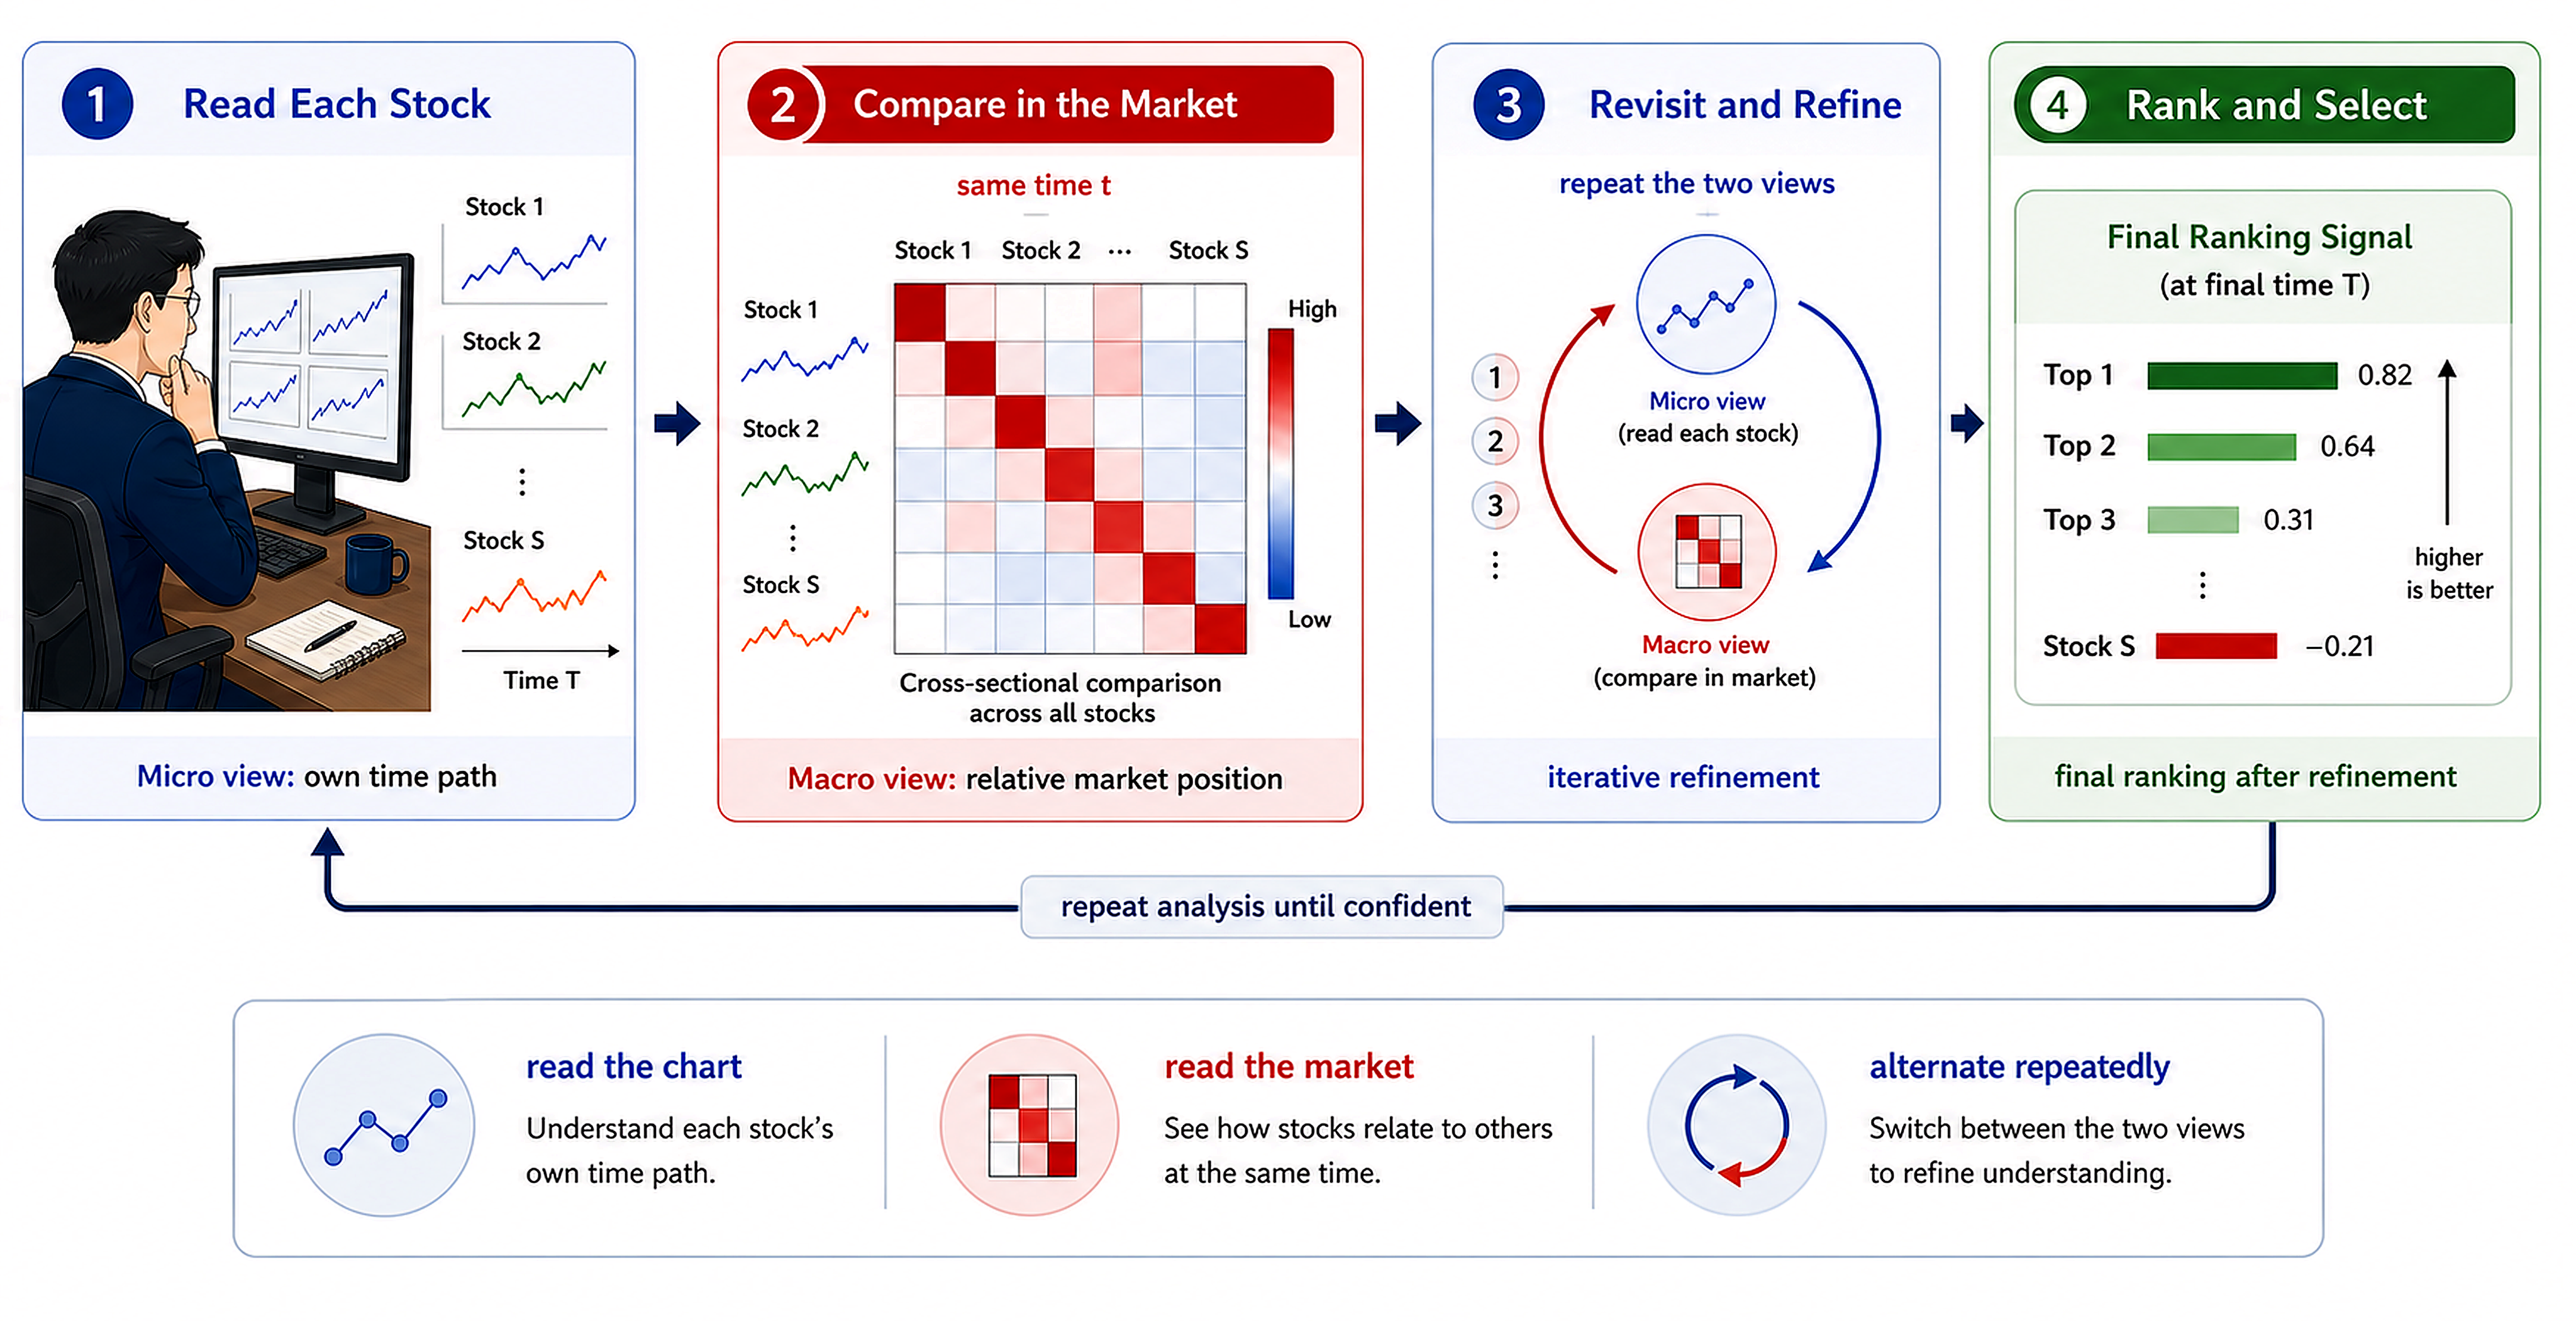
\includegraphics[width=\linewidth]{figures/fig_trader.png}
\caption{交易者的双视角认知过程。沿时间轴读单股走势（Micro 视角）、沿截面轴在全市场中横向比较
（Macro 视角），并在两个视角间反复切换、迭代精炼，直至给出最终排序。本文将这一过程显式建模为可
堆叠的 \msq{} Block。}
\label{fig:trader}
\end{figure}

深度学习选股已从早期只建单股时序的模型（RNN、CNN）发展到同时建模时间与截面两个维度的双轴架构。
然而现有双轴方法普遍存在两点不足。其一，\textbf{两个视角只走一遍}：先看自身趋势、再看截面位置，
一次顺序流程结束便输出结果。但这两类信号是\emph{相互依赖}的——时序模式的解读依赖截面语境（同样
“下跌 5\%”在牛市与崩盘中含义迥异），而截面位置的判断又依赖时序轨迹（“今天偏高”是持续爬升还是
刚刚冲顶）；单趟处理时，两个视角都在“尚不知道对方结论”的情况下各自计算，没有互相修正的机会。
其二，\textbf{时间维被过早压扁}：许多方法在末端把整段时间窗压缩成单一向量再做预测，丢失了窗口内
逐日的状态，而短期动量恰恰是 A 股最稳定的信号之一。

基于以上观察，我们的核心主张是：要解开上述这种相互依赖，必须把两个视角\textbf{显式解耦}、再
\textbf{迭代地互相精炼}，而非单趟顺序走一遍。据此我们提出 \msqa{}（Micro--Macro Alpha Engine）：
把沿时间轴的微观注意力（Micro）与沿截面轴的宏观注意力（Macro）封装成一个可堆叠的 \msq{} Block，
通过多层堆叠让两个视角递归地互相深化（对应图~\ref{fig:trader} 中第三格的反复重读）。其余设计——
全程保留 $(S,T,D)$ 表征并对每个时间步密集监督、不显式注入市场状态——在第~\ref{sec:method} 节展开。

此外，低信噪比带来一个贯穿全文的反直觉现象：\emph{预测越准并不代表选股越赚}。例如同一次训练中，
按“验证集 IC 最高”选出的检查点（ep34）样本外累计仅 $+67.2\%$，而验证 IC 居中的 ep13 反而取得
最高的 $+170.9\%$——验证 IC 与样本外收益系统性背离。这一现象及其对模型选择准则的影响在第~\ref{sec:select}
节详述。

\noindent\textbf{\heiti 两项核心设计创新.}
\begin{itemize}
  \item \textbf{（双轴模块化与迭代重读）} 把双轴交互封装成一个可堆叠、可逐轴关断探查的特征提取原语
        \msq{} Block，通过多层堆叠让 Micro 与 Macro 递归地互相精炼。本文不主张发明双轴建模的思想（该思想
        已有清晰谱系，见第~\ref{sec:rw-dual} 节），而是把它整理成一个\emph{可解剖、可迭代}的单元。该创新由
        双轴消融、堆叠深度扫描与等参数量加宽对照支撑（第~\ref{sec:pillars}、\ref{sec:depth} 节）。
  \item \textbf{（保留 $(S,T,D)$ 与密集时间监督）} 全程保留股票$\times$时间$\times$隐藏维的三维表征、不在末端
        压扁时间轴，并对窗口内每个时间步施加密集的截面排序监督。其中\emph{保留时间维}（表征设计）与\emph{密集
        监督}（目标设计）是两个可分开的选择，本文用一个固定架构、仅把损失从全窗口改成只监督末步的受控消融，
        隔离并\emph{证实}了密集监督本身的贡献——两个口径都显著优于只监督末步、误差带不重叠（第~\ref{sec:abl-dense} 节）。
\end{itemize}

\noindent\textbf{\heiti 实验与方法学贡献.}
\begin{itemize}
  \item \textbf{（评测协议与选点失效发现）} 提出一套统一评测协议（最优检查点 $+$ 多种子 $+\,\pm60$pp 方差
        红线），并据此得到一个可迁移的发现：低信噪比下验证集 IC 与样本外收益\emph{反向}，标准的 best-valid-IC
        选点准则会系统性选到泛化更差的模型（第~\ref{sec:select} 节）。
  \item \textbf{（Macro 是学出来的截面去噪器——一个经验发现）} 注意力分析、带权收缩扫描与全市场共动检验共同
        表明：训练后的 Macro 表现得像一个\emph{自适应截面去噪器}，把每只股票的预测往一群数据驱动的相关同伴
        共识上收、压低单股特异噪声。其软分组与申万行业的互信息（NMI）仅 $0.23$，参照的\emph{不是行业均值}、
        也不是外部关系图（第~\ref{sec:macro} 节）。这是对一个为横截面参照而设计的模块的\emph{事后}解释，而非
        预设的设计创新，并在 James--Stein / 经验贝叶斯收缩框架下获得自然诠释。
  \item \textbf{（实证与诚实归因）} 在 CSI300 与 13 个代表性方法的对照下，\msqa{} 在最优检查点协议下收益居前
        （seed42 $+170.9\%$、多种子 $+155\%$，高于所有重现 baseline，如 RSR $+94.5\%$、对抗式 ALSTM
        $+78.9\%$）。但本文的产出不止于收益，更在于穿过方差红线后仍成立的少数稳健结论，以及"低信噪比下，
        怎么训练、怎么选点比架构本身更重要"这一判断。
\end{itemize}

\noindent\textbf{\heiti 全文组织.}
第~\ref{sec:related} 节梳理相关工作；第~\ref{sec:data} 节交代数据、任务与特征工程 pipeline；
第~\ref{sec:method} 节详述 \msqa{} 的结构与训练；第~\ref{sec:exp} 节给出实验设置、统一评测协议、主对照、
两个创新的消融证据与 Macro 作用机制；第~\ref{sec:discuss} 节讨论局限；第~\ref{sec:conclusion} 节总结。

% ================================================================ 2 相关工作
\section{相关工作与预备知识}\label{sec:related}

\subsection{单股票时序建模}\label{sec:rw-seq}
最早一类方法将每只股票视为一条独立的时间序列。循环网络（LSTM~\cite{lstm}、GRU）及其注意力增强版
（ALSTM~\cite{alstm}）沿时间轴建模个股历史，预测其未来收益或涨跌；频域方法 SFM~\cite{sfm} 把隐状态
分解到不同频率分量上以刻画多周期模式；卷积类方法则用一维卷积沿时间轴提取局部形态。三者分别以循环、
卷积、注意力作为时序建模的归纳偏置，但共享同一个更强的假设——\emph{单股票、纯时序}：一只股票的未来
主要由其自身历史决定。在以\emph{相对排序}为目标的选股任务中，这一假设遗漏了横截面信息，而"同一天其他
股票表现如何"恰恰是定义"这只股票是否强势"的参照系。

\subsection{双轴依赖建模：图先验 vs 数据驱动}\label{sec:rw-dual}
为引入横截面信息，一类工作沿时间轴与股票轴两个维度同时建模。按"股票间关系来自何处"，可分为两支。

\textbf{\heiti 图先验。} 这一支显式给定股票关系图。RSR~\cite{rsr} 用行业、供应链等关系构造邻接矩阵，
并通过 Temporal Graph Convolution 把相关股票的表征互相平滑；HIST~\cite{hist} 进一步区分预定义概念与
从数据中挖掘的隐含概念。其关系是\emph{外生}的，依赖关系数据的覆盖与时效，且关系图通常是静态的。

\textbf{\heiti 数据驱动。} 这一支不预设关系，而用注意力在股票轴上自行学习个股间的相互影响。
DTML~\cite{dtml} 将市场状态与个股表征一并送入其所谓的 data-axis Transformer（即股票轴），让股票彼此 attend；
MASTER~\cite{master} 在时间轴与股票轴上交替做注意力，并用市场状态调制个股特征。相近的还有
StockMixer~\cite{stockmixer}（用 MLP-mixing 在时间、特征、股票三维交替混合）与通用多变量时序模型
Crossformer~\cite{crossformer}（Two-Stage Attention 分别在时间与变量维做注意力）。

本文沿数据驱动这条线展开，并以 MASTER 作为最直接的对比对象。\emph{双轴依赖建模}这一思想由上述工作
共同确立，本文不主张其首创。与 MASTER 的关键区别在于处理方式：MASTER 走\emph{单趟}流程（时间轴一次、
股票轴一次，随后压扁时间维做预测），而本文把双轴交互整理成一个\emph{可堆叠、可逐轴关断}的单元，全程
保留 $(S,T,D)$ 表征、采用因果时序，并对每个时间步施加密集的截面排序监督。

\subsection{监督方式与时间表征压缩}\label{sec:rw-sup}
本文第二个设计选择关乎\emph{如何对待时间窗口}，这里单独交代其文献背景。许多时序选股模型在预测前会把整个回看
窗口\emph{压成一个末端向量}：循环网络取最后一个隐状态 $h_T$、注意力模型（如 MASTER）在股票轴交互后对时间维
做池化或只保留末步——随后只在这个压缩表征上预测、也只有末步状态承担监督。这其实把两件\emph{本可分开}的设计
混在了一起：一是\textbf{表征设计}（representation）——要不要压扁时间维，还是保留完整的 $(S,T,D)$；二是
\textbf{目标设计}（objective）——是只监督末步，还是对窗口内每个时间步都密集监督。前者关乎模型能否在每一层都
让时序与截面信息充分交织，后者关乎训练时的梯度密度。

本文的第二个创新正落在这一对选择上：\emph{保留 $(S,T,D)$ 表征}（不在中途压扁时间维）并\emph{对所有时间步密集
监督}。由于二者常被一并采用、难以归因，我们在实验中把它们拆开测量——固定架构、只把损失从"全窗口监督"换成
"只监督末步"，以隔离密集监督本身的贡献（§\ref{sec:abl-dense}）。这一拆解视角，是本文相对上述压缩式做法的主要
定位差异。

\subsection{训练范式}\label{sec:rw-train}
除架构外，训练目标与正则化在低信噪比下同样关键。AdvALSTM~\cite{advalstm} 在输入或隐层加入对抗扰动以
提升泛化；TRA~\cite{tra} 设置多个"交易模式"并用最优传输把样本路由到不同模式，缓解单一模式的过拟合；
RSR~\cite{rsr} 直接优化 pairwise 排序损失，而非逐股回归。这些为低信噪比专门设计的训练范式，在
第~\ref{sec:main} 节的失效诊断中表现出与任务更高的契合度——其与任务的匹配程度，往往比架构是否精巧更
能决定最终成败。

\paragraph{归纳偏置与双轴处理}
从更高层看，上述方法可由两个维度刻画（表~\ref{tab:cnn-track}）：其一是时序建模的归纳偏置（循环 / 卷积
/ 注意力）；其二是如何处理时间轴与股票轴这两个维度——是在一趟前向中\emph{融合}（fuse）走过，还是把两轴
\emph{解耦}（decouple）后反复交织。绝大多数已有方法属于前者；本文的切入点是后者：解耦双轴并迭代精炼。

\begin{table}[H]
\centering
\caption{时序归纳偏置 $\times$ 双轴处理方式。多数方法在单趟前向中融合两轴；本文将两轴解耦并迭代。}
\label{tab:cnn-track}
\begin{tabularx}{\linewidth}{l>{\raggedright\arraybackslash}X>{\raggedright\arraybackslash}X}
\toprule
时序归纳偏置 & 代表方法 & 双轴处理方式 \\
\midrule
循环（RNN）    & ALSTM, DTML            & 单趟融合 \\
卷积/混合（CNN/MLP） & 时序卷积, StockMixer & 单趟融合 \\
注意力（Attention） & MASTER；\msqa{}（本文） & MASTER 单趟融合；\textbf{本文解耦 $+$ 迭代} \\
\bottomrule
\end{tabularx}
\end{table}

\paragraph{记号约定}
本文用粗体大写表示矩阵 / 张量（如 $\bm{X}$），粗体小写表示向量（如 $\bm{x}$），普通小写表示标量。
股票数记 $S$，时间步 $T$，特征维 $F$，隐藏维 $D$。完整记号见表~\ref{tab:notation}。

% ================================================================ 3 数据、任务与特征工程
\section{数据、任务与特征工程}\label{sec:data}
量化任务里数据处理流程是可信度地基：它直接决定有没有未来信息泄露、标签是否对齐、特征是否可交易、回测
是否可信。本节先把任务形式化，再把从原始行情到特征张量 $\bm{X}\in\mathbb{R}^{S\times T\times F}$、从未来收益
到标签 $\bm{Y}\in\mathbb{R}^{S\times T}$ 的完整数据流交代清楚；表~\ref{tab:pipeline} 是该流程的一页总览。

\subsection{任务定义：截面排序}\label{sec:data-task}
每个交易日 $d$ 的输入是一个面板 $\bm{X}_d\in\mathbb{R}^{S_d\times T\times F}$（$S_d$ 为当日有效股票数、
$T{=}8$ 为回看窗口、$F{=}35$ 为每日特征维），标签是 $\bm{Y}_d\in\mathbb{R}^{S_d\times T}$。模型对窗口内
\emph{每个}时间步 $t$ 都输出一个截面分数，训练时全部监督（§\ref{sec:m-head}）；\emph{推理时只取窗口末步}
$\hat{\bm{Y}}_{:,T}$ 作为当日交易信号，按分数对全市场降序排序、取头部构成持仓。也就是说，模型学的不是"涨
多少"，而是"今天这只票在全市场里相对强弱排第几"——这正是低信噪比下更可学、也更贴近选股决策的目标。

\subsection{数据来源与股票池}\label{sec:data-universe}
\textbf{\heiti 原始数据.} A 股日频研究面板，时间跨度 2017-01 至 2026-05。完整历史训练需要兼容本仓库数据协议的外部面板；公开数据路线使用 BaoStock 作为历史底座，使用 AKShare / efinance 做公开增强，历史量比由成交量派生 proxy 回填，估值、市值与行业等字段走可用快照，资金流历史则尝试通过东财风格接口补齐并记录覆盖率。二者仍是不同数据源：公开缓存可无密钥审计，但不等价于研究面板；当前公开缓存的自由流通换手仍可能为 proxy，历史资金流字段也可能因公开端点不可稳定审计而退化为中性占位，因此部分输入信号弱于研究实验。字段含
量价（开 / 高 / 低 / 收 / 成交量 / 成交额）、每日基本面（\texttt{daily\_basic}：换手率、量比、PE/PB/PS 等）
与资金流（\texttt{moneyflow}：各档买卖单金额）。\emph{未使用}新闻文本、研报或外部事件数据——这一限制及其
背后的判断见 §\ref{sec:discuss}。

\textbf{\heiti 股票池.} 训练在\emph{沪深 300} 成分股上（大盘、信号相对干净的标注池），回测 / 评测在\emph{流动性
最高的约 1000 只}（top1000）上。top1000 按\emph{每月末流通市值}排序取前 1000（仿中证 1000 lite 的动态调样），
逐月重选，并剔除 ST 股与北交所（\texttt{.BJ}）股。动态月度调样使股票池随时间滚动、用的是每月末时点信息、不前视，
一定程度上缓解了固定成分股的幸存者偏差。需要提醒：训练（沪深 300）与回测（top1000）的股票池\emph{并不一致}，
这是一次"大盘训练、更广股票池部署"的跨域泛化考验，其影响列入局限（§\ref{sec:discuss}）。

\subsection{特征工程流程}\label{sec:data-feat}
特征不是一张静态清单，而是一条按时间生成的流水线。\textbf{\heiti（1）按股票分组.} 所有滚动特征按
\texttt{groupby(ts\_code)} 在单只股票的时间序列上计算，不跨股票混入彼此信息。\textbf{\heiti（2）只用当日及以前.} 任一交易日
$t$ 的特征只读 $[\,\cdot,t\,]$ 区间的数据（动量、均线偏离、波动率等滚动量的窗口右端点即为 $t$），不触碰未来；
基本面与资金流字段为日频、按交易日对齐，假设\emph{盘后}即可获得、用于次日建仓。\textbf{\heiti（3）七组共
35 维.} 多尺度动量、均线偏离、波动率、K 线形态、成交量、每日基本面、资金流共 $35$ 个因子，其中前五组（量价）
为 Alpha158~\cite{qlib} 子集、基本面取自 \texttt{daily\_basic}、资金流 2 个为自构。完整分组、来源标注与逐因子
公式见附录~\ref{sec:features}（表~\ref{tab:features}）。最终每只股票每个交易日得到一个 $35$ 维向量，按 $T{=}8$
天的窗口堆叠成 $\bm{X}\in\mathbb{R}^{S\times T\times F}$。

\subsection{缺失值、异常值与标准化}\label{sec:data-norm}
\textbf{\heiti 样本完整性.} 构造窗口时要求每只股票在 $[t{-}T{+}1,\,t]$ 内\emph{每一天}都有数据、且标签有效，
任一缺失即\emph{当日整只剔除}（不前向填充、不补零），保证 $\bm{X}$ 内不混入插补值；停牌、上市未满一个窗口、
基本面 / 资金流缺失的样本因此自然落选。\textbf{\heiti 标准化.} 用\emph{逐日截面 robust z-score}：每个交易日
仅在\emph{当日横截面}内做
\begin{equation}\label{eq:zscore}
\tilde{x} = \mathrm{clip}\!\Big(\frac{x-\mathrm{median}}{1.4826\,\mathrm{MAD}},\,-5,\,+5\Big),
\end{equation}
其中 median / MAD 均在当日截面上估计，裁剪阈值 $\pm5$，标准化后仍为空的位置填 $0$。这一选择有两重好处：
$(x-\mathrm{median})/(1.4826\,\mathrm{MAD})$ 比普通 $z$-score 对涨跌停、个股尖刺更鲁棒；而\emph{逐日、只在当日
截面内}做（既不跨日、也不在训练 / 全量上估计统计量），从构造上杜绝了"全量标准化"那类未来信息泄露。

\subsection{标签构造与无泄漏约束}\label{sec:data-label}
窗口内每个时间步 $t$ 的原始标签是该股的\emph{次日可交易收益}
\begin{equation}\label{eq:label}
r_{s,t} = \frac{\mathrm{close}_{s,\,t+2}}{\mathrm{close}_{s,\,t+1}} - 1,
\qquad y_{s,t}=\mathrm{zscore}_{\text{当日截面}}(r_{s,t}),
\end{equation}
即"第 $t$ 日收盘后出信号、第 $t{+}1$ 日收盘买入、第 $t{+}2$ 日收盘卖出"，严格符合 A 股 T+1（当日买入须次日
才能卖）。窗口内\emph{每一天}都按此构造标签并做当日截面 $z$-score，这正是密集监督的标签来源（§\ref{sec:m-head}）；
特征只用建仓前可得信息、标签只取窗口之后的收益，时间上不重叠。\textbf{\heiti 一处需如实说明的口径差.}
式~\eqref{eq:label} 的标签是\emph{收盘到收盘}（close-to-close），而回测建仓用的是\emph{次日开盘价}成交
（§\ref{sec:setup}）——二者并不完全一致。我们保留这一差异并据实标注：它会让样本外收益与训练标签之间存在
一层执行价偏移，是回测数字的已知近似来源之一，而非泄漏。

\begin{table}[H]
\centering
\caption{数据处理与特征工程流程总览。}
\label{tab:pipeline}
\begin{tabularx}{\linewidth}{l>{\raggedright\arraybackslash}X}
\toprule
环节 & 做法 \\
\midrule
原始数据   & A 股日频，2017-01 至 2026-05；量价 + \texttt{daily\_basic} + \texttt{moneyflow}；无新闻 / 外部数据 \\
股票池     & 训练=沪深 300；回测=top1000（每月末按流通市值取前 1000、动态调样）；剔除 ST、北交所 \\
特征构造   & \texttt{groupby(ts\_code)} 滚动，仅用 $[\cdot,t]$；7 组共 35 维（公式见附录~\ref{sec:features}） \\
缺失 / 异常 & 窗口内任一缺失则当日整只剔除（不插补）；标准化后残余空值填 $0$ \\
标准化     & 逐日截面 robust z-score $(x{-}\mathrm{med})/(1.4826\,\mathrm{MAD})$，裁剪 $\pm5$（式~\ref{eq:zscore}） \\
标签       & $r_{s,t}{=}\mathrm{close}_{t+2}/\mathrm{close}_{t+1}{-}1$，当日截面 $z$-score；T+1 合规（式~\ref{eq:label}） \\
切分       & 训练 2017-01\,$\sim$\,2023-12 / 验证 2024-01\,$\sim$\,2025-06 / 测试 2025-07\,$\sim$\,2026-05 \\
回测 universe & top1000、开盘成交（与训练池沪深 300 不同，见 §\ref{sec:data-universe}） \\
\bottomrule
\end{tabularx}
\end{table}

% ================================================================ 4 方法
\section{方法}\label{sec:method}

\msqa{} 用于 A 股截面选股：给定过去 $T$ 个交易日、$S$ 只股票的日频特征，预测每只股票次日的
\emph{截面相对强弱}，并按强弱排序选取持仓。模型是一个始终保持「股票 $\times$ 时间 $\times$ 隐藏维」
三维表征的 Transformer，核心是用两种注意力\emph{交替}提炼股票的两类信息——其在\emph{时间轴}上的
近期轨迹，与其在\emph{截面轴}上相对全市场的当日位置；下文统称这两条轴为\emph{双轴}。如图~\ref{fig:method}，
模型分三步：(i) 将原始特征投影为隐表征；(ii) 堆叠 $L$ 个结构相同的 \msq{} Block，每个 Block 依次
沿双轴做注意力与位置前馈；(iii) 用一个共享线性头在每个时间步输出预测分，取末步分数排序选股。
整个过程不在中途压扁任何维度，$(S,T,D)$ 表征贯穿始终。

\begin{figure}[t]
\centering
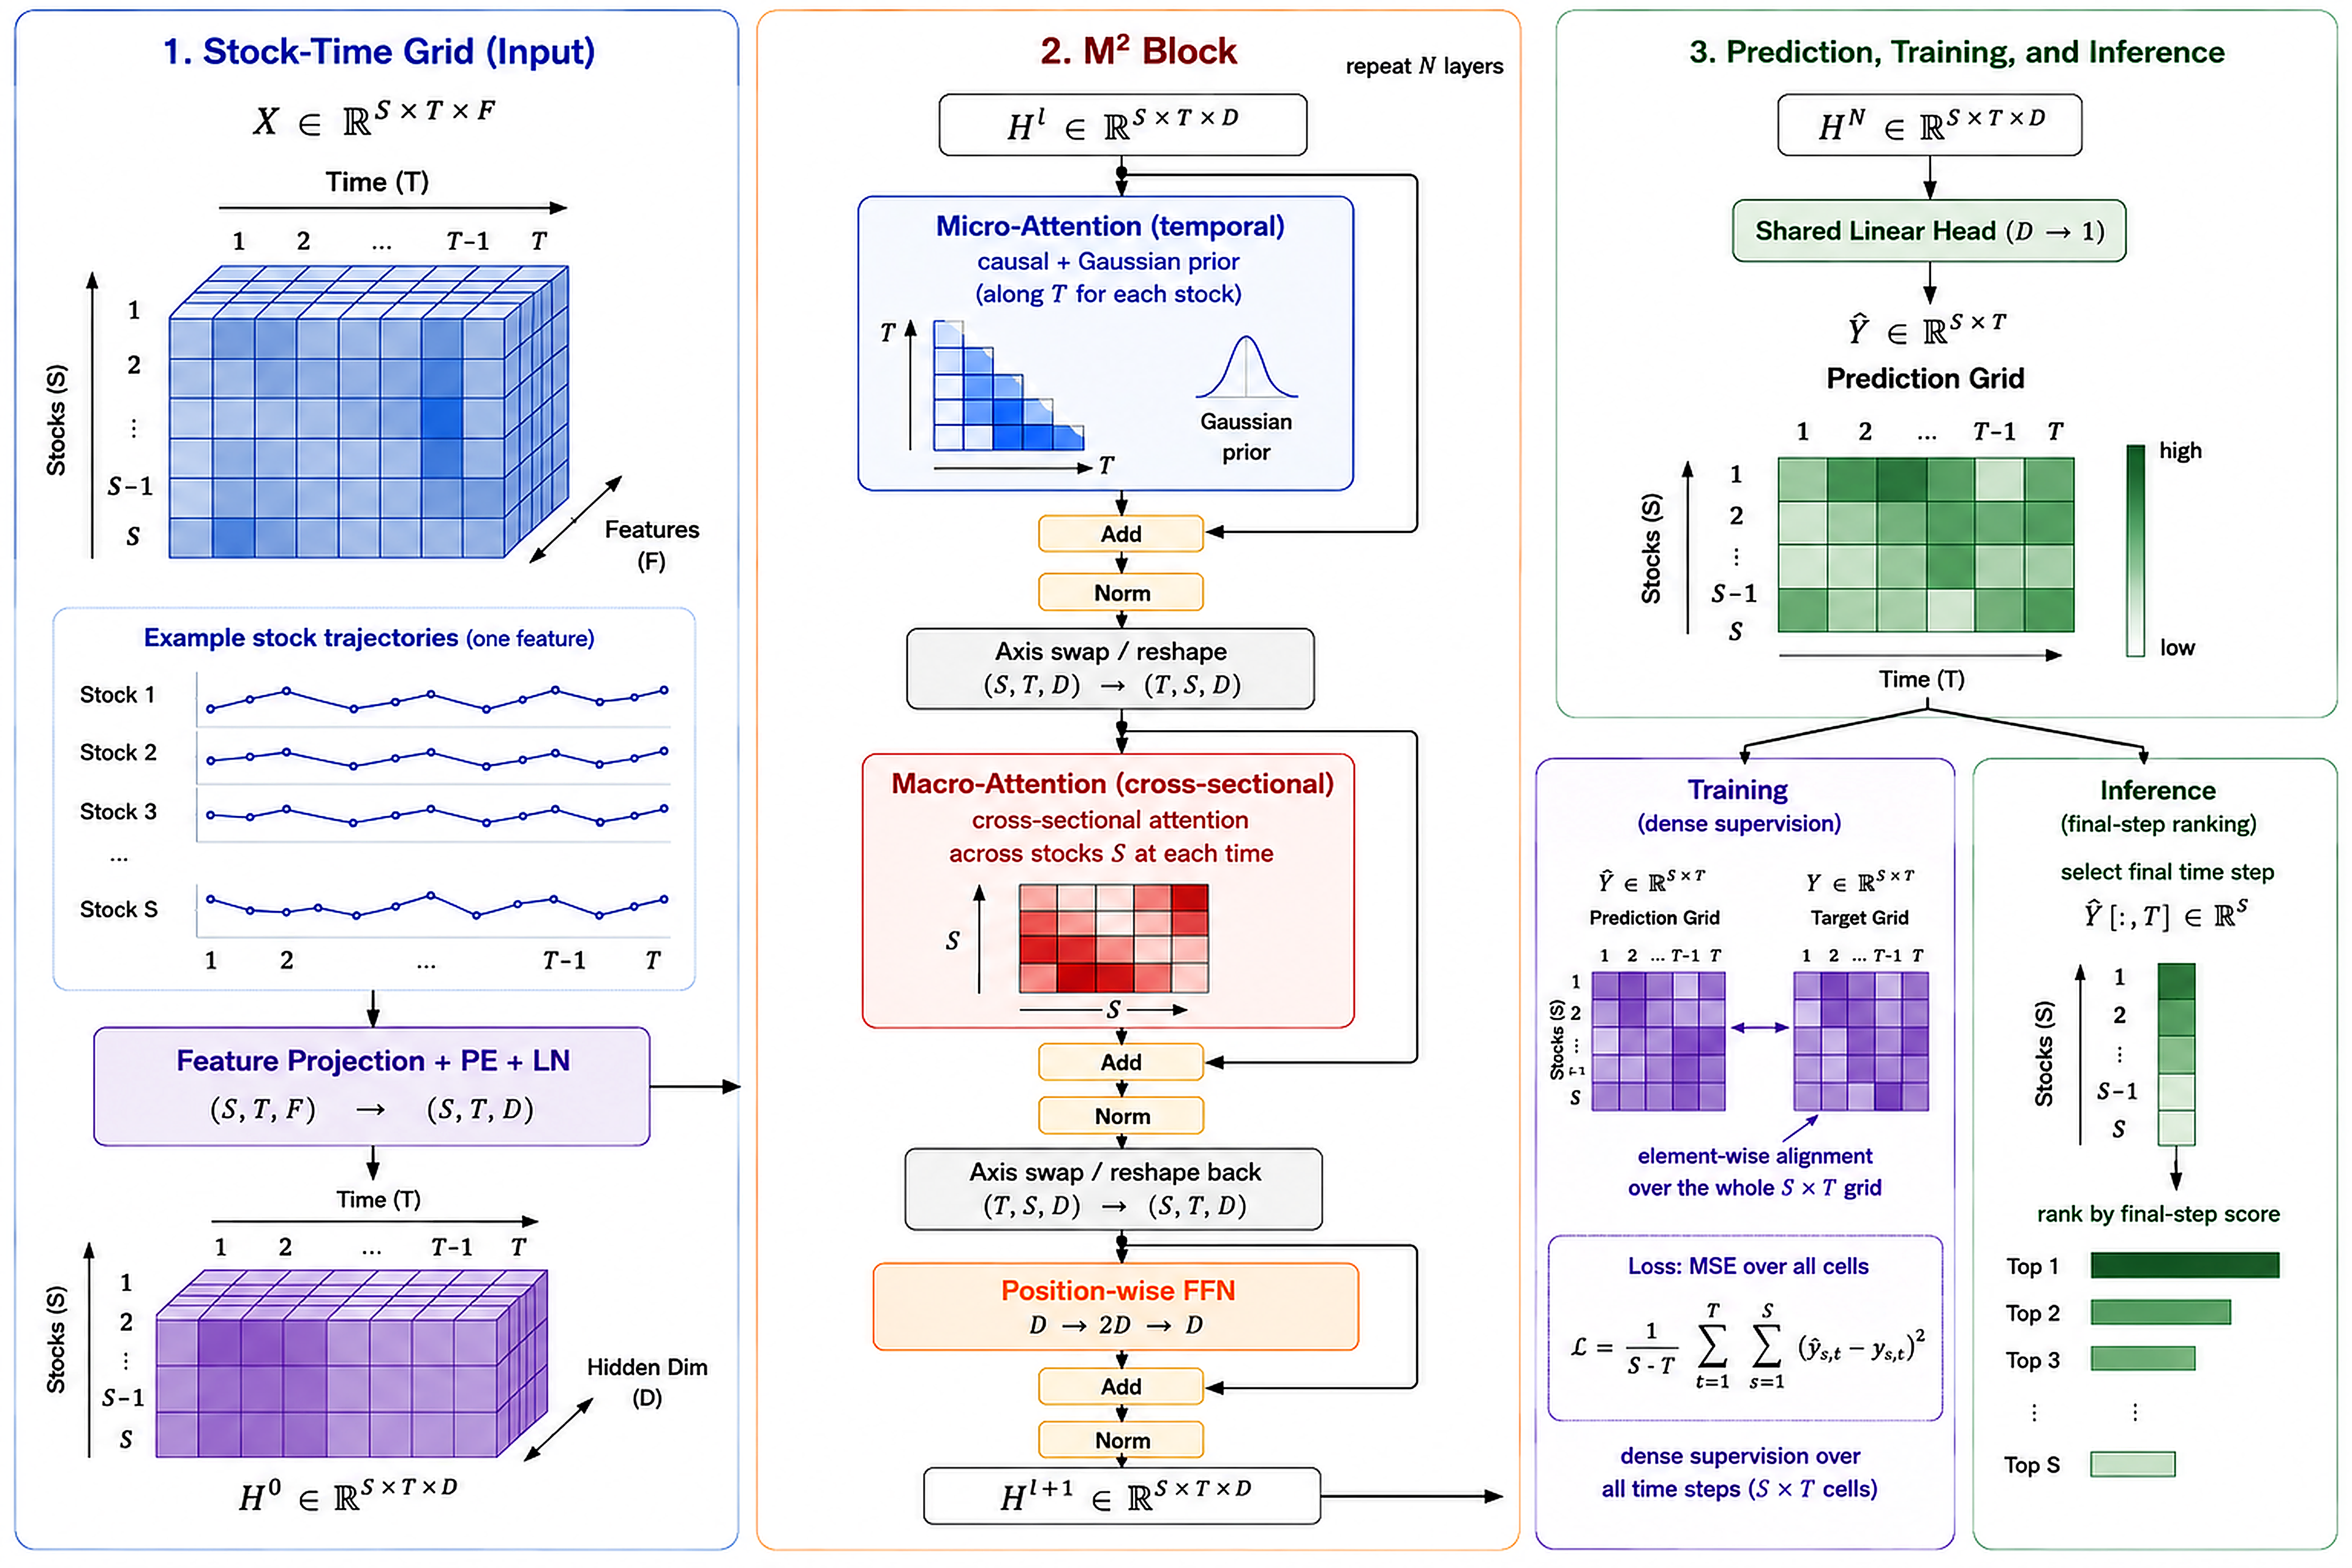
\includegraphics[width=\linewidth]{figures/fig_method.png}
\caption{\msqa{} 总体结构。左：输入为“股票 $\times$ 时间 $\times$ 特征”网格，经特征投影 $+$ 位置编码 $+$
层归一化得到 $\bm{H}^{(0)}$。中：$L$ 层 \msq{} Block，每层依次做 Micro（时间轴因果注意力 $+$ 高斯近邻
先验）、Macro（截面轴注意力）、位置前馈 FFN（$D\!\to\!2D\!\to\!D$），各子层残差 $+$ 归一化，并在两轴
之间转置张量。右：共享线性头逐时间步输出预测网格 $\hat{\bm{Y}}$，训练时对整张 $S\times T$ 网格密集监督，
推理时取末步分数排序选股。}
\label{fig:method}
\end{figure}

\subsection{设计动机：双轴依赖与迭代重读}\label{sec:m-intuition}
判断一只股票是否值得买，交易者通常同时依赖双轴上的两类信息：这只票\emph{自己这段时间的轨迹}（时间轴），
以及它\emph{今天在全市场的相对位置}（截面轴）。只看轨迹会忽略当日市场风格是否偏好这类票，只看截面位置
又会丢失它最近是在加速还是见顶。

更关键的是，这两类信息\emph{互相依赖}：要判断“今天排第几”，得先理解每只票各自的轨迹，否则截面位置
没有语义；要解读“这段轨迹意味着什么”，又得参照当日市场语境——同样的跌幅在崩盘与牛市里含义相反。
单趟顺序处理（先做完一个轴再做另一个）解不开这种循环依赖：第一遍处理时间轴时截面语境尚未可知，
第一遍处理截面轴时用的又是未经截面校准的时序表征。

因此我们用 $L$ 层结构相同的 Block 让双轴\emph{迭代}地互相重读：每一层 Macro 输出的截面信息会通过
残差连接流入下一层 Micro 的输入，使后者在已知当日市场语境的前提下重新解读该股票的时间轨迹；下一层
的 Macro 又拿到这份经语境校准的时序表征，再次更新截面位置。这里“组合”是结构（两个轴都跑了），
“迭代”是行为（后一遍是在前一遍输出上重读，而非重复运算）。堆叠带来的增益是否确实源于这一迭代行为、
而非单纯的参数增多，由第~\ref{sec:depth} 节的实验检验。

\subsection{输入表示与特征投影}\label{sec:m-input}
记一个交易截面的输入为 $\bm{X}\in\mathbb{R}^{S\times T\times F}$：$S$ 只股票、回看窗口 $T$ 个交易日、
每日 $F$ 维特征（记号汇总见表~\ref{tab:notation}）。先经一层逐 (股票,时间) 共享的线性投影把特征维
映射到模型维 $D$，叠加时间轴的（正弦）位置编码 $\bm{P}$ 并层归一化，得到初始隐表征
\begin{equation}\label{eq:input}
\bm{H}^{(0)} = \mathrm{LN}\big(\mathrm{Proj}(\bm{X}) + \bm{P}\big)\ \in\ \mathbb{R}^{S\times T\times D}.
\end{equation}
默认配置直接以原始特征 $\bm{X}$ 入投影。

\begin{table}[H]
\centering
\caption{记号与符号表。}
\label{tab:notation}
\begin{tabularx}{\linewidth}{l>{\raggedright\arraybackslash}X}
\toprule
符号 & 含义 \\
\midrule
$S,\ T,\ F,\ D$ & 股票数、回看时间步数、输入特征维、模型隐藏维 \\
$\bm{X}\in\mathbb{R}^{S\times T\times F}$ & 输入面板（股票 $\times$ 时间 $\times$ 特征） \\
$\bm{H}^{(\ell)}\in\mathbb{R}^{S\times T\times D}$ & 第 $\ell$ 层 Block 的隐表征（$\ell=0,\dots,L$） \\
$\bm{H}^{(\ell)}_{s}\in\mathbb{R}^{T\times D}$ & 第 $s$ 只股票的时序表征切片（Micro 输入） \\
$\bm{H}^{(\ell)}_{:,t}\in\mathbb{R}^{S\times D}$ & 第 $t$ 个时间步的截面切片（Macro 输入） \\
$\bm{Q},\bm{K},\bm{V}$ & 注意力的查询/键/值投影；$d_k$ 为每个头的维度 \\
$\sigma$ & Micro 高斯近邻先验的带宽（baseline $\sigma{=}4$） \\
$L$ & \msq{} Block 堆叠层数（baseline $L{=}3$） \\
$\hat{\bm{Y}}\in\mathbb{R}^{S\times T}$ & 逐时间步截面预测；末步 $\hat{\bm{Y}}_{:,T}$ 为交易信号 \\
\bottomrule
\end{tabularx}
\end{table}

\subsection{\msq{} Block：双轴注意力}\label{sec:m-block}
一个 \msq{} Block 顺序串联三个子层——Micro（时间轴因果注意力）、Macro（截面轴注意力）、位置前馈
FFN——每个子层都带残差连接与（post-）层归一化。设第 $\ell$ 层输入为 $\bm{H}^{(\ell)}$。

\comp{Micro（时间轴，因果 $+$ 近邻先验）}
Micro 对\emph{每一只股票独立地}在时间轴上做多头自注意力~\cite{transformer}，刻画其自身轨迹。为防止信息
泄漏，注意力被约束为\emph{因果}的（第 $i$ 步只能看 $j\le i$ 的历史）；并借鉴 Gaussian
Transformer~\cite{gausstransformer} 的高斯先验思想，在注意力 logits 上叠加一个加性的\emph{时间距离
高斯先验}（单一带宽 $\sigma$，见下式），使模型偏向近邻时间步。对股票 $s$，记其表征序列为 $\bm{H}^{(\ell)}_{s}\in\mathbb{R}^{T\times D}$，
\begin{equation}\label{eq:micro}
\mathrm{Micro}\big(\bm{H}^{(\ell)}_{s}\big)=\mathrm{softmax}\!\Big(\frac{\bm{Q}_s\bm{K}_s^{\top}}{\sqrt{d_k}}+\bm{B}\Big)\bm{V}_s,
\qquad
\bm{B}_{ij}=\begin{cases}\exp\!\big(-\dfrac{(i-j)^2}{2\sigma^2}\big), & j\le i,\\[8pt] -\infty, & j>i,\end{cases}
\end{equation}
其中 $\bm{Q}_s,\bm{K}_s,\bm{V}_s$ 由 $\bm{H}^{(\ell)}_{s}$ 线性投影得到。$\bm{B}$ 的下三角项是随时间
距离衰减的正偏置（越近的过去权重越高），上三角的 $-\infty$ 实现因果屏蔽。

\comp{Macro（截面轴，软共识）}
Macro 在\emph{每一个时间步独立地}让所有股票互相做多头自注意力，刻画个股在当日全市场中的相对位置。
实现上把张量在股票轴与时间轴之间转置，对时间步 $t$ 的截面 $\bm{H}_{:,t}\in\mathbb{R}^{S\times D}$，
\begin{equation}\label{eq:macro}
\mathrm{Macro}\big(\bm{H}_{:,t}\big)=\mathrm{softmax}\!\Big(\frac{\bm{Q}_t\bm{K}_t^{\top}}{\sqrt{d_k}}\Big)\bm{V}_t.
\end{equation}
这里不施加任何掩码——每只股票都能 attend 当日的所有股票，得到的是横截面上的一种\emph{软共识}，而非
基于行业或供应链的硬关系图。第~\ref{sec:macro} 节通过可解释性实验分析 Macro 实际学到的内容，并为这一
设计选择提供依据。

\comp{FFN、残差与归一化}
最后逐 (股票,时间) 位置过一层前馈网络 $\mathrm{FFN}(\bm{h})=\bm{W}_2\,\mathrm{ReLU}(\bm{W}_1\bm{h})$，
其中 $\bm{W}_1:\mathbb{R}^{D}\!\to\!\mathbb{R}^{2D}$、$\bm{W}_2:\mathbb{R}^{2D}\!\to\!\mathbb{R}^{D}$。
三个子层统一采用残差 $+$ 后置归一化：
\begin{equation}\label{eq:residual}
\bm{H}\ \leftarrow\ \mathrm{LN}\big(\bm{H}+\mathrm{Sublayer}(\bm{H})\big),\qquad
\mathrm{Sublayer}\in\{\mathrm{Micro},\ \mathrm{Macro},\ \mathrm{FFN}\},
\end{equation}
依次应用 Micro、Macro、FFN 后即得本层输出 $\bm{H}^{(\ell+1)}$。

\subsection{堆叠与迭代精炼}\label{sec:m-stack}
$L$ 层结构相同的 Block 顺序堆叠，$\bm{H}^{(\ell+1)}=\mathrm{Block}\big(\bm{H}^{(\ell)}\big)$，
$\ell=0,\dots,L-1$。由于每个子层都带残差连接，第 $\ell{+}1$ 层 Micro 的输入已经累积了第 $\ell$ 层
Macro 注入的截面信息：它不再处理“裸的”原始时序，而是在已知当日市场语境的前提下重新解读该股票的时间
轨迹——这正是第~\ref{sec:m-intuition} 节所述的迭代重读。堆叠因此不是把同一运算重复 $L$ 次，而是让两个
互相依赖的视角在残差通道上交替收敛。

一个自然的疑问是：堆叠的增益会不会只是因为参数变多了？我们在第~\ref{sec:depth} 节用两组对照排除这一
可能：一是加宽表示维度 $D$（只加参数、不加迭代层），收益很快饱和（$D{=}128$ 与 $256$ 持平），达不到加深
的高度；二是扫描堆叠层数 $L\in[1,5]$，加深仍在抬升、只是增速放缓，符合“迭代逐层精炼、收益递减”而非“参数
越多越好”的预期。

整个堆叠过程不压扁时间维，$(S,T,D)$ 表征贯穿始终，为逐时间步的密集监督保留完整信息。

\subsection{预测头、标签与训练目标}\label{sec:m-head}
最末层表征 $\bm{H}^{(L)}$ 经一个所有 (股票,时间) 共享的线性头映射到标量，得到预测网格
\begin{equation}\label{eq:head}
\hat{\bm{Y}} = \bm{H}^{(L)}\bm{w} + b\ \in\ \mathbb{R}^{S\times T}.
\end{equation}
标签 $\bm{Y}\in\mathbb{R}^{S\times T}$ 的每个元素 $y_{s,t}$ 是股票 $s$ 在第 $t$ 日的\emph{次日截面
$z$-score 收益}（在当日横截面内做标准化，使监督信号本身就是“相对强弱”而非绝对涨跌）。训练时对整张
$S\times T$ 网格施加\emph{密集监督}，baseline 采用均方误差
\begin{equation}\label{eq:loss}
\mathcal{L}=\frac{1}{S\,T}\sum_{s=1}^{S}\sum_{t=1}^{T}\big(\hat{y}_{s,t}-y_{s,t}\big)^2 .
\end{equation}
密集监督让窗口内每个时间步都成为一次训练信号，大幅提高了梯度密度。推理时只取末步分数
$\hat{\bm{Y}}_{:,T}\in\mathbb{R}^{S}$ 作为当日交易信号，按分数对股票降序排序、取前若干只构成持仓
（回测口径见第~\ref{sec:setup} 节）。除均方误差外，我们在第~\ref{sec:objective} 节系统比较了排序损失
与分类损失等不同训练目标。

\subsection{实现细节与默认配置}\label{sec:m-impl}
\textbf{\heiti 模型.} baseline 配置为：回看窗口 $T{=}8$ 个交易日、模型维 $D{=}128$、堆叠 $L{=}3$ 层、
Micro 多头数 $4$ / Macro 多头数 $2$、FFN 扩张倍数 $2$、dropout $0.1$、高斯带宽 $\sigma{=}4$、正弦位置
编码、post-norm、块内顺序 Micro$\to$Macro。默认\emph{不使用}行业先验（industry attention）；行业先验
连同 PE 变体、稀疏 Macro 等，作为变体在第~\ref{sec:exp} 节与附录中讨论。市场向量由 3 个市场指数（上证
综指、沪深 300、创业板指）在 5 个回看尺度上聚合得到，仅在用到市场
信息的变体中启用。权重采用 Xavier 初始化。

\textbf{\heiti 训练.} 以\emph{一个交易日的全部股票}为一个 batch；优化器 AdamW（学习率 $10^{-5}$、
权重衰减 $10^{-4}$），梯度按范数裁剪到 $5.0$；baseline 不使用学习率调度（调度策略作为附录消融）。
最多训练 $40$ 个 epoch，并按\emph{验证集 IC} 早停（patience $=10$）。每个配置用 3 个随机种子
（42 / 123 / 2024）独立训练。数据划分、标准化与无泄露处理见第~\ref{sec:setup} 节。

% ================================================================ 4 实验
\section{实验}\label{sec:exp}

% ---------------- 4.1
\subsection{实验设置与统一评测协议}\label{sec:setup}

\textbf{\heiti 数据与任务.} 数据来源、股票池、特征 pipeline、标准化与无泄漏的标签构造已在第~\ref{sec:data}
节统一交代（总览见表~\ref{tab:pipeline}）：约 $35$ 维量价 / 基本面 / 资金流特征、逐日截面 robust z-score、
截面排序标签、按时间划分为训练 2017-01\,$\sim$\,2023-12 / 验证 2024-01\,$\sim$\,2025-06 / 测试 2025-07\,$\sim$\,2026-05。
本节只补回测与评测口径。

\textbf{\heiti 回测与评测.} 训练在沪深 300 成分股上，回测在流动性最高的约 1000 只股票（top1000；已剔除
流动性差的 ST 股与北交所股）上。交易策略沿用统一回测模板并加分散约束（下称\emph{本文回测策略}）：等权持有
$n{=}10$ 只，每日从预测分最高的 top-100 买入、把持仓中跌出 top-200 的卖出，单一行业仓位上限 $20\%$，开盘价
成交，双边手续费 $0.13\%$，初始资金 100 万元。预测质量用 IC（信息系数，当日预测与次日实际收益的截面相关系数）、
RankIC（其秩相关版本）与 ICIR（IC 序列的均值 $/$ 标准差，衡量稳定性）衡量；回测用累计收益、年化、
夏普、最大回撤，与市场指数（上证综指、沪深 300）及简单 MLP 基线对比（第~\ref{sec:main} 节）。图~\ref{fig:loss}
是 baseline 的训练 / 验证损失：训练损失稳步下降、验证损失基本持平，是低信噪比金融数据的常见形态，也预示
验证侧指标与样本外表现会脱节（第~\ref{sec:select} 节）。

\begin{figure}[H]
\centering
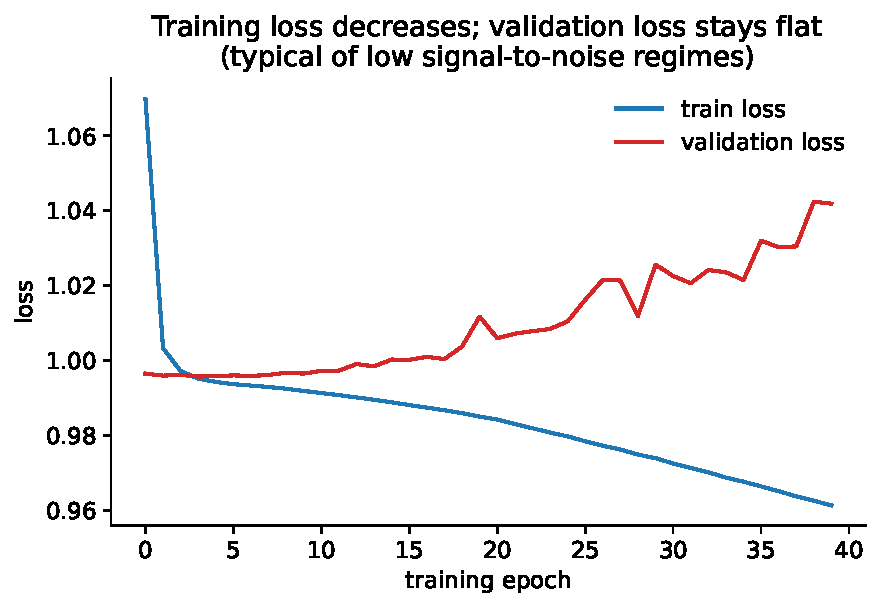
\includegraphics[width=0.62\linewidth]{figures/fig_loss.pdf}
\caption{baseline 的训练与验证损失随 epoch 的变化。训练损失稳步下降，验证损失基本持平——低信噪比金融
数据下的常见形态，也预示验证侧指标与样本外表现会脱节（第~\ref{sec:select} 节）。}
\label{fig:loss}
\end{figure}

\textbf{\heiti 统一评测协议.} 每个配置同时报两个数。\textbf{(i) 最优 ckpt}\bestckpt{}：在逐 epoch 存的检查点
（checkpoint，简称 ckpt）里按\emph{测试}收益取最高的一个；它借用了本不可见的测试集信息，是 oracle 上界，只
衡量能力天花板与跨种子稳定性、不可部署。\textbf{(ii) 验证段选点}：用验证集挑检查点，是诚实、可部署的数。关键
结论一律给多种子 $\text{mean}\pm\text{std}$（seed 42/123/2024），并设\textbf{方差红线} $\approx\pm 60$pp——
同一配置仅因种子与检查点选择即可产生的收益波动量级（见第~\ref{sec:select} 节），相差不到红线即按噪声处理。
\textbf{\heiti 判据约定.} 本文统一以\emph{误差带 $=$ 多种子 $\text{mean}\pm1\,\text{std}$}（$n{=}3$）为准：两个配置的误差
带\emph{不重叠}才视为超出种子噪声的真实差异，重叠则按同量级噪声处理。须强调 $n{=}3$ 偏小，这是\emph{工程判读}
而非严格统计检验，只支撑"是否明显分离"的定性结论。另外，\bestckpt{} 是在\emph{已存}检查点网格上取测试最优，
不同配置若存档网格疏密不一，其可比性会打折——故本文把网格不等长的对比降格为\emph{印证性}证据（如
附录~\ref{sec:abl-dense}），主判据以网格一致或验证选点口径的对照为准。
表~\ref{tab:protocol} 是 base 在两种口径下的读数模板。

\begin{table}[H]
\centering
\caption{统一评测协议下的读数模板（以 base 为例）。\bestckpt{} = 最优 ckpt（上界）。}
\label{tab:protocol}
\begin{tabular}{lcccc}
\toprule
配置 & seed42 & seed123 & seed2024 & mean$\pm$std \\
\midrule
base（最优 ckpt\bestckpt） & +170.9\% & +166.0\% & +128.6\% & $+155\pm19$\% \\
base（验证段选点）         & +55\%    & +117\%   & $-3$\%      & \msd{+56}{60}\% \\
\bottomrule
\end{tabular}
\end{table}

% ---------------- 4.2
\subsection{选点失效与跨种子方差}\label{sec:select}
在低信噪比的截面任务上，同一个配置仅仅换一个随机种子、或换一个检查点，收益就能相差上百个百分点。这个
噪声的量级，是判读一切架构对比的前提：差异小于它，就无从区分"真效应"与"换了个种子"。

\textbf{\heiti 设置.} 以 baseline（$L{=}3$、$D{=}128$、$\sigma{=}4$）做两组对照，回测口径与第~\ref{sec:setup}
节一致（top1000 池、开盘成交、双边费 $0.13\%$、测试期 2025-07 至 2026-05）。第一组固定 seed42，逐 epoch 存
检查点并各自回测，考察一次训练内收益随 epoch 的走势是否与验证 IC 同向；第二组固定其余配置、只改种子（42 /
123 / 2024），分别按\emph{验证段选点}与\emph{最优 ckpt} 两种规则取数，度量种子带来的波动。

\textbf{\heiti 结果.} 一次训练内，验证 IC 随 epoch 单调上升（$0.020\to0.027$），测试收益却在 ep13 见顶后
持续回落，二者 Pearson 相关 $-0.75$（图~\ref{fig:ic-return}）。按"验证 IC 最高"选检查点会选到 ep34——
样本外最差的一端，而真正最好的 ep13 验证 IC 并不突出。只改种子时，验证段选点的三个种子收益为 $-3\%$、
$+55\%$、$+117\%$（mean $+56\%$、std $\pm60$pp）；同样三个种子改用最优 ckpt 则为 $+171\%$ / $+166\%$ /
$+128\%$（mean $+155\%$、std 收窄到 $\pm19$pp）。seed2024 的 $-3\%$ 并非模型更差，而是这次训练的验证选点
恰好落在泛化差的检查点上。

\textbf{\heiti 分析.} 这里有三层意思。其一，验证 IC 不能用来选检查点——它与样本外收益反向，常规
early-stopping 在此适得其反。更一般地说：在信噪比这么低的环境里，一个指标涨上去，本身往往是过拟合的信号、
而非能力变强的证据——验证段短、噪声大，后期 IC 的攀升多半是模型在拟合验证集的噪声（与图~\ref{fig:loss} 验证
损失不降一致）。IC 这种点估计相关性，在高噪声下已经不是“样本外能力”的可靠代理，“更准”未必“更赚”。其二，
种子与选点合起来的收益波动约 $\pm60$pp，超过后面多数架构改动的效应。这两点定下全篇的判读规则：关键结论
一律给最优 ckpt $+$ 多种子 mean$\pm$std，配置之间相差不到 $\pm60$pp 即按噪声处理、不声称孰优——文献中大量
基于单次运行报告的“架构提升”，很可能就落在这条红线之内。其三，既然指标本身会在噪声里骗人，“训练该优化
什么、部署该信什么”就得结合场景来定，而非盲目最大化 IC：第~\ref{sec:objective} 节正会看到，直接盯着排序
（IC 类目标）的损失方差反而更大，真正稳的是回归与分类。各配置的收益分布见图~\ref{fig:variance}。

\begin{figure}[H]
\centering
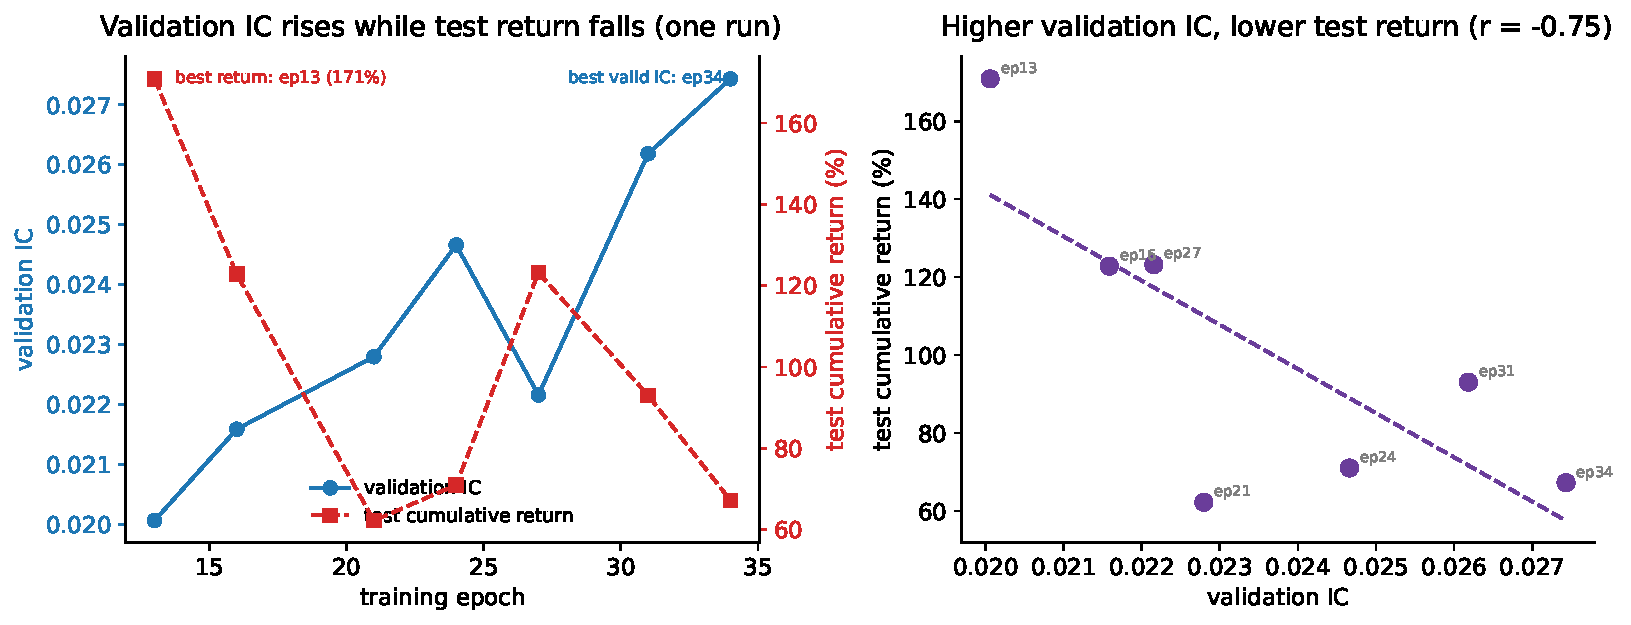
\includegraphics[width=\linewidth]{figures/fig_ic_return.pdf}
\caption{验证 IC 与样本外收益的反向关系（baseline，seed42）。左：同一次训练逐 epoch，验证 IC 持续上升，
测试累计收益在早期见顶后回落。右：每个检查点为一点，验证 IC 越高、样本外收益越低，Pearson $r=-0.75$；
按"验证 IC 最高"选点（ep34）恰好落在收益最差的一端。}
\label{fig:ic-return}
\end{figure}

\begin{figure}[H]
\centering
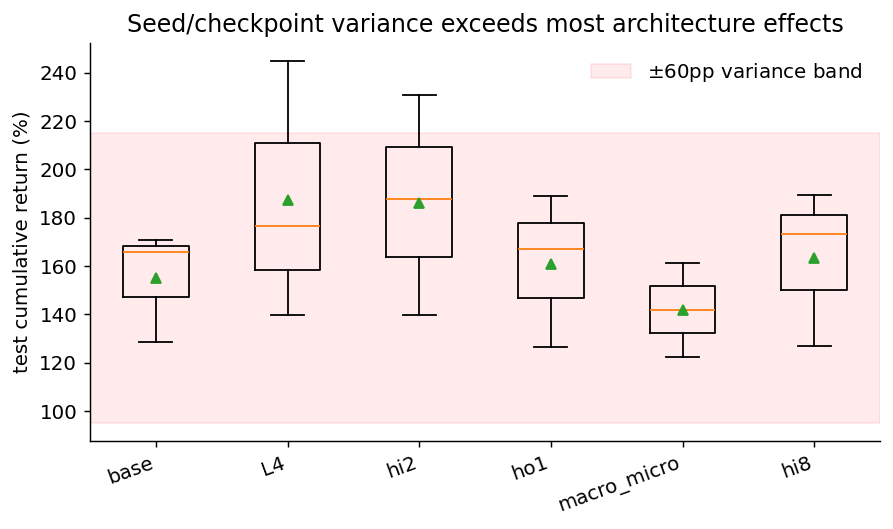
\includegraphics[width=0.92\linewidth]{figures/fig_variance.png}
\caption{各配置在多种子上的最优-ckpt 收益分布（箱线图，三角为均值），叠加以 base 为中心的 $\pm 60$pp
方差红线带。base 与多数架构变体（更深的堆叠、不同的 Micro / Macro 注意力头数、调换的子层顺序）种子间
波动彼此交叠，且都落在红线带量级内——配置间差异在很大程度上无法与种子噪声区分。}
\label{fig:variance}
\end{figure}

% ---------------- 4.3
\subsection{主对照与失效诊断}\label{sec:main}

\subsubsection{主对照}\label{sec:main-cmp}
\textbf{\heiti 设置.} 13 个代表性方法与 \msqa{} 在同一面板上对照：相同的 $35$ 维特征、相同的数据划分、
相同的回测策略（第~\ref{sec:setup} 节），测试期 2025-07 至 2026-05。baseline 各按原始设定训练、取验证段
选点的单种子（seed42）结果，\msqa{} 取最优 ckpt。沪深 300 被动持有是市场基准，逐点 MLP（不建模任何时序
与截面关系）是"无结构"下界。

\textbf{\heiti 结果.} \msqa{}（最优 ckpt）以 $+170.9\%$、夏普 $2.99$ 居首（表~\ref{tab:main}）。为低信噪比
设计的训练范式派次之——RSR $+94.5\%$、对抗式 AdvALSTM $+78.9\%$、TRA $+63.2\%$；经典时序模型（Transformer /
LSTM / ALSTM / GRU）落在 $+20\%\sim+49\%$；被改成截面排序的金融特化模型（HIST / MASTER / DTML / SFM）垫底，
$+3\%\sim+23\%$。沪深 300 被动持有是 $+24.8\%$：训练范式派和 \msqa{} 明显跑赢大盘，GRU、MASTER、DTML、SFM
反而不及指数。

\textbf{\heiti 分析.} 排在前面的是为低 SNR 设计的 ranking / 对抗范式，不是容量更大的经典架构——收益来自
对任务的适配，不是堆参数。这张表不能照字面排名次：baseline 是单种子、\msqa{} 是 oracle 上界，口径不对称，
而单种子收益本身就有 $\pm60$pp 抖动（第~\ref{sec:select} 节）。逐点 MLP 是最好的提醒——它不建模任何时序与
截面关系，最优 ckpt 下仍有 $+98.3\%$、反超多数专用 baseline；在 oracle 上界下，强特征加选点已经能解释相当
一部分收益。因此这张表只读作 oracle 上界下的能力对照；多种子、可部署口径的逐项结果见第~\ref{sec:pillars} 节及之后。

\begin{table}[H]
\centering
\caption{主对照：统一回测口径（本文回测策略，seed42）。\msqa{} 为最优 ckpt（上界），baseline 为单种子。}
\label{tab:main}
\begin{tabular}{llccc}
\toprule
类别 & 模型 & test 累计 & Sharpe & 最大回撤 \\
\midrule
\textbf{本文} & \textbf{\msqa{}（最优 ckpt）} & \textbf{+170.9\%} & \textbf{2.99} & $-14.7\%$ \\
\midrule
\multirow{3}{*}{训练范式派}
 & RSR        & +94.5\% & 2.07 & $-22.3\%$ \\
 & AdvALSTM   & +78.9\% & 2.10 & $-27.0\%$ \\
 & TRA        & +63.2\% & 1.63 & $-18.3\%$ \\
\midrule
\multirow{4}{*}{经典时序}
 & Transformer & +48.8\% & 1.49 & $-14.1\%$ \\
 & LSTM        & +37.9\% & 1.52 & $-14.7\%$ \\
 & ALSTM       & +33.8\% & 0.91 & $-36.4\%$ \\
 & GRU         & +20.2\% & 1.17 & $-10.7\%$ \\
\midrule
\multirow{4}{*}{金融特化}
 & HIST   & +23.2\% & 0.79 & $-28.6\%$ \\
 & MASTER & +9.6\%  & 0.47 & $-37.4\%$ \\
 & DTML   & +4.9\%  & 0.36 & $-28.5\%$ \\
 & SFM    & +3.3\%  & 0.31 & $-34.7\%$ \\
\midrule
\multirow{2}{*}{简单基准}
 & MLP（逐点，无时序） & +98.3\% & 2.12 & $-17.1\%$ \\
 & 沪深 300 指数（被动持有） & +24.8\% & 1.79 & $-7.8\%$ \\
\bottomrule
\end{tabular}
\end{table}

\subsubsection{失效诊断}\label{sec:main-diag}
金融特化模型集体垫底，一种可能是被改成截面排序目标后性能下降。

\textbf{\heiti 设置.} 按各自论文的原始目标与信号忠实复现三者——MASTER 用 5 日收益 MSE、DTML 用涨跌 BCE、SFM
用逐股价格 MSE——在同一回测口径下评测（表~\ref{tab:faithful}）。

\textbf{\heiti 结果.} 忠实目标下三者依旧偏低（表~\ref{tab:faithful}）：MASTER $-19.8\%$、DTML $+4.5\%$、
SFM $+9.0\%$，与表~\ref{tab:main} 里被改成 ranker 的版本同样差。关键是否定信号——不是回测口径或费用吃掉了
收益：三者全程验证 IC 都贴在 $-0.01$ 到 $0$ 之间（MASTER $-0.011\sim-0.006$、DTML $-0.008\sim-0.002$、
SFM $-0.005\sim-0.001$），约等于零、略偏负，即预测分数与次日截面收益几乎不相关。IC$\approx 0$ 说明它们在
A 股压根没学到可用的截面信号。

\textbf{\heiti 分析.} 既然按各自论文的原始目标忠实复现、并非被改成 ranker，IC 仍接近零，就排除了"目标被
改坏"这一解释，失效落在架构与任务的结构性不匹配——这些模型的目标与归纳偏置本就不适配 A 股低 SNR 的截面
排序。逐个看：\textbf{MASTER}（$-19.8\%$，唯一亏损）靠市场引导门控、用整体市场状态调制个股表示，而 A 股
市场因子噪声大、风格切换快，门控易锁到伪市场信号、把噪声当结构放大——这与第~\ref{sec:macro} 节互为镜像：
Macro 有用是因为收敛到少数稳健的共涨共跌簇，MASTER 把"整个市场均值"当锚、锚错了方向。\textbf{DTML}
（$+4.5\%$）训练目标是涨跌二分 BCE，而 A 股日频涨跌接近五五开、二分标签几乎不含信息，与第~\ref{sec:objective}
节 BCE 直接崩到 $-6\%$ 同理，标签层先天丢了截面强弱。\textbf{SFM}（$+9.0\%$）做频率分解加逐股价格 MSE，前提
是股价有可分解的稳定周期成分；A 股价格非平稳、个股特异噪声大，分解出的多是噪声谐波，而逐股 MSE 优化的是
单股价格拟合、与横截面相对排序正交。三者的失效汇聚到同一结论：在低 SNR 的截面排序任务上，带强弱信号的
ranking / 对抗范式（表~\ref{tab:main} 的训练范式派）才有效，这些为别的目标设计的架构迁不过来。

\textbf{\heiti 边界.} 这是开箱忠实迁移的失败（论文默认超参、单种子 seed42），不等于模型本身不行——在各自
原始的市场、时段、评测口径下论文结果成立。MASTER、DTML 两条失效机制有本文自己的实验旁证（第~\ref{sec:macro}
节的 Macro 锚、第~\ref{sec:objective} 节的 BCE 崩）；SFM 那条更多是架构原理的推断，本文未做专门的频率分解
消融。

\begin{table}[H]
\centering
\caption{忠实 baseline（各自论文目标，seed42）。}
\label{tab:faithful}
\begin{tabular}{lcc}
\toprule
模型（忠实目标） & test 累计 & Sharpe \\
\midrule
MASTER（5 日收益 MSE） & $-19.8\%$ & $-0.34$ \\
DTML（涨跌 BCE）       & $+4.5\%$  & $+0.34$ \\
SFM（逐股价格 MSE）    & $+9.0\%$  & $+0.47$ \\
\bottomrule
\end{tabular}
\end{table}

% ---------------- 4.3
\subsection{双轴消融}\label{sec:pillars}
模型的能力压在两根轴上：Micro 沿时间轴读单股自己的轨迹，Macro 沿截面轴把它和同伴横向比较（第~\ref{sec:method}
节）。设计若成立，拆掉任意一根，收益都该明显下降；若某根其实冗余，拆掉它收益不变、甚至更高。

\textbf{\heiti 设置.} 两种拆法。去掉 Macro 这根截面轴后，股票之间不再横向交互，模型退化成一条只沿时间轴
走的单股序列模型；把 Micro 读时间轴的方式从因果自注意力换成单向 LSTM 后，时间轴还在，但读法从"窗口内
全局注意力"退回"逐日循环"。其余配置、数据划分、回测口径都与 base 相同，每个变体跑种子 123/2024、取最优
ckpt（口径见第~\ref{sec:select} 节）。

\textbf{\heiti 结果.} 两根轴缺一不可（表~\ref{tab:pillars}、图~\ref{fig:pillars}）。base 是 $+155\pm19\%$，关掉
Macro 降到 $+109\pm7\%$（$-46$pp），Micro 换 LSTM 降到 $+111\pm10\%$（$-44$pp）。这 $45$pp 上下的降幅与种子方差
红线（$\pm60$pp）同量级，单看一次运行难辨真伪；但在最优-ckpt 多种子口径下，两个变体都低于 base、误差带与
base 不重叠，是真实效应。验证段选点口径下，关掉 Macro 的个别种子会选到泛化差的检查点、收益低至接近零（与
base 验证选点 seed2024 落到 $-3\%$ 同一机制，§\ref{sec:select}），这是选点假象而非模型真降到零；换最优 ckpt 口径
才看清它稳在 $+109\%$，比 base 系统性低，但远没归零。

\textbf{\heiti 分析.} 两根轴掉收益，各有可追溯的机制。关 Macro 的机制将在第~\ref{sec:macro} 节专门展开：Macro
干的活是把过度极端的预测往横截面共识上收（$59\%$ 的股票被拉近行业均值）；撤掉它，个股的极端打分不再被同伴
校正，排序就更容易被单股噪声带跑偏。Micro 换 LSTM 的降幅与之相当，差在读时间轴的方式——因果自注意力让窗口里任一天
都能直接回看此前任一天，LSTM 只能把历史压进一个隐状态逐步往后递，远端信息一路衰减。还要排除一个混淆：换
LSTM 的同时也丢了 Micro 的高斯近邻先验；但单独去掉高斯先验，收益落在噪声带内（附录~\ref{sec:abl-micro}），
所以这 $44$pp 主要记在"时间轴怎么读"上，不在高斯先验。两根轴撤掉后误差带都与 base 分离、机制又各自可追溯，说明它们不是
互为冗余的备份，而是收益真正各自依赖的支柱。

\begin{table}[H]
\centering
\caption{双轴支柱消融（test 累计收益，最优 ckpt、多种子）。三个配置均为种子 42/123/2024
（$n{=}3$）；关 Macro 与 Micro 换 LSTM 的误差带均与 base 不重叠。}
\label{tab:pillars}
\begin{tabular}{lcccc}
\toprule
配置 & seed42 & seed123 & seed2024 & mean$\pm$std \\
\midrule
base（完整）        & $+170.9$ & $+166.0$ & $+128.6$ & $\mathbf{+155\pm19}$ \\
关 Macro（无截面交互） & $+105.9$ & $+119.2$ & $+102.3$ & $+109\pm7$ \\
Micro 换 LSTM       & $+121.5$ & $+97.6$  & $+115.2$ & $+111\pm10$ \\
\bottomrule
\end{tabular}
\end{table}

\begin{figure}[H]
\centering
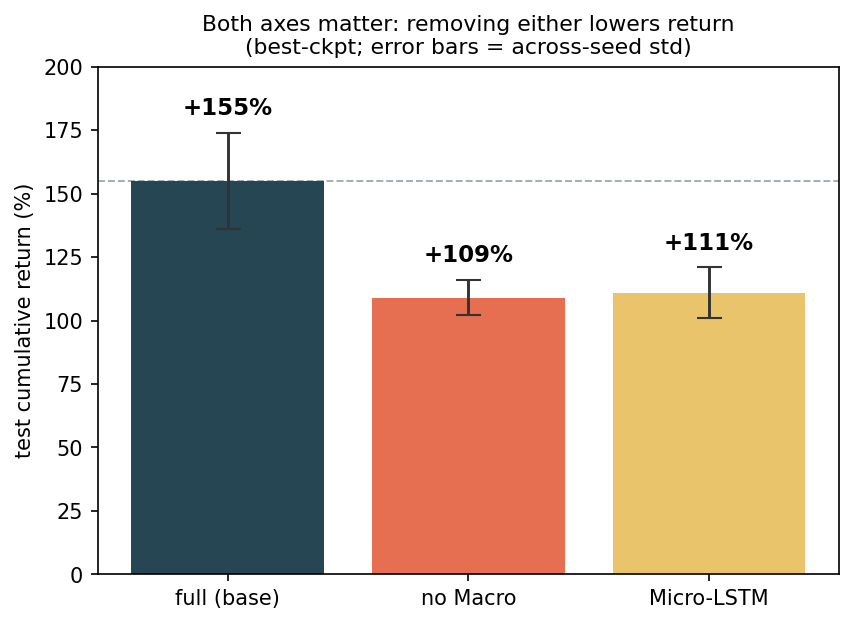
\includegraphics[width=0.62\linewidth]{figures/fig_pillars.png}
\caption{双轴支柱（最优 ckpt，误差棒为种子标准差）。关掉 Macro 或把 Micro 换成 LSTM 后，收益误差带都
与 base 不重叠——下降是超出种子噪声的真实效应。}
\label{fig:pillars}
\end{figure}

% ---------------- 4.5
\subsection{堆叠深度}\label{sec:depth}
第~\ref{sec:m-stack} 节用堆叠 \msq{} Block 让双轴迭代重读。堆叠的增益可能来自这种迭代，也可能只是层数多、
参数多；层数扫描用来区分这两种解释。

用第~\ref{sec:m-stack} 节的记号把"迭代"写明确：从输入表征 $\bm{H}^{(0)}$ 出发，深度 $L$ 就是反复施加同一个
Block 的轮数，
\begin{equation}\label{eq:iter}
\bm{H}^{(L)}=\underbrace{\mathrm{Block}\circ\cdots\circ\mathrm{Block}}_{L\ \text{层}}\big(\bm{H}^{(0)}\big),
\qquad
\bm{H}^{(\ell+1)}=\mathrm{Block}\big(\bm{H}^{(\ell)}\big)=\mathrm{FFN}\!\big(\mathrm{Macro}\,(\mathrm{Micro}(\bm{H}^{(\ell)}))\big),
\end{equation}
每个子层都带残差。要点在残差让两轴交替"重读"对方的最新结论：第 $\ell{+}1$ 层的 Micro 读到的 $\bm{H}^{(\ell)}$
已经累积了上一层 Macro 注入的截面语境，而这一层的 Macro 又读到 Micro 刚精炼过的时序表征。所以加深一层不是把
同一映射多算一遍，而是让 Micro / Macro 在彼此的最新输出上多迭代一轮、把表征 $\bm{H}$ 逐层精炼——$L$ 直接控制
"重读几轮"。深度实验扫的就是这个 $L$。

\textbf{\heiti 设置.} 固定其余配置（$D{=}128$、$\sigma{=}4$、Micro / Macro 头数与基址结构不变），只改堆叠
层数 $L\in\{1,2,3,4,5\}$，每个 $L$ 用 3 个种子独立训练、逐 epoch 回测取最优 ckpt。为了分开"迭代"与"参数
变多"两种解释，另取加宽表示维度 $D$ 的扫描（$D\in\{64,128,256\}$，附录~\ref{sec:abl-arch}，同为最优-ckpt
多种子口径）作对照——加宽是"只加参数、不加迭代层"，若增益主要来自参数量，加宽也该一路涨。

\textbf{\heiti 结果.} 表~\ref{tab:depth} 与图~\ref{fig:depth} 给出深度曲线。深度总体有益：单层 $L{=}1$ 收益
最低（$+126\pm36\%$），$L{=}2$ 起跃升至 $+165\%$ 一线，$L{=}4$、$L{=}5$ 进一步抬到 $+187\%$、$+201\%$。但各深度
误差带（$\pm19$ 到 $\pm44$pp）大幅交叠，$L{=}3$（base）在均值上甚至略低于 $L{=}2$；逐种子看，$L{=}4$ 在三个
种子上都高于 $L{=}3$，但 $L{=}5$ 与 $L{=}4$ 孰高因种子而异（seed2024 上 $L{=}5$ 反而最高）。

\textbf{\heiti 分析.} 深度有益的方向与迭代假说一致：每多一层（式~\eqref{eq:iter} 多迭代一轮），Micro 就在上一
层 Macro 注入的截面语境下重新解读时序，两轴的相互依赖被多解开一层。最能说明问题的是 $L{=}1\to2$ 这一跳
（$+126\to+165$、$+39$pp，是整条曲线最大的一步）：单层时两轴只各算一遍、谁也不知道对方的结论，到两层，Micro
才第一次在 Macro 的截面语境上重读——迭代从无到有，收益就跳了一档；这正是"重读"本身在起作用、而非单纯多了一层
参数的最直接证据。增益在 $L{=}4$ 后趋缓，符合"迭代有收敛点"——双轴交替重读几次已足够解开依赖；再加深，更大容量在低信噪比、
数据有限下倾向过拟合、放大种子方差（误差带随 $L$ 变宽）。

那增益会不会只是层数多、参数多？加宽 $D$ 的对照（附录~\ref{sec:abl-arch}）给出否定的旁证：从 base（$L{=}3$、
$D{=}128$、$+155\%$）出发往两个方向加同一批参数——加在\emph{宽度}上（$D{:}128\to256$）收益从 $+155\%$ 走平到
$+154\%$（饱和、落在误差带内），加在\emph{深度}上（$L{:}3\to4\to5$）却继续抬到 $+187\%$、$+201\%$。同样是多塞
参数，加在宽度上不再有用、加在深度上还在涨，说明深度的增益不是"参数更多、容量更大"本身，而是每多一层带来的
又一轮双轴重读——这正是"堆叠即迭代重读"的设计要点。当然，最干净的"等参数量、单宽层 vs 多薄层"对照仍留作
后续工作。这条深度曲线同样落在方差主线里——连堆叠层数这样根本的选择，效应量级也与种子 / 选点噪声相当
（第~\ref{sec:select} 节）。

\begin{figure}[H]
\centering
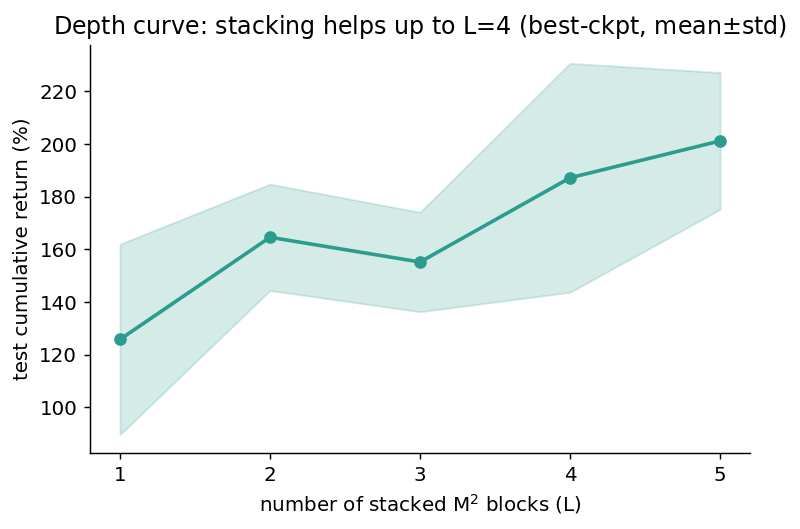
\includegraphics[width=0.62\linewidth]{figures/fig_depth.png}
\caption{深度曲线：测试累计收益随堆叠 \msq{} Block 层数 $L$ 的变化（最优 ckpt，三种子 mean$\pm$std 阴影）。
深度总体有益（$L{=}1$ 最低、更深更高），但误差带大幅交叠、无干净单一甜区。}
\label{fig:depth}
\end{figure}

\begin{table}[H]
\centering
\caption{深度曲线（test 累计收益，最优 ckpt、三种子 mean$\pm$std）。}
\label{tab:depth}
\begin{tabular}{lcccc}
\toprule
层数 $L$ & seed42 & seed123 & seed2024 & mean$\pm$std \\
\midrule
L1 & $+75.0$  & $+156.7$ & $+145.7$ & $+126\pm36$ \\
L2 & $+145.6$ & $+155.6$ & $+192.6$ & $+165\pm20$ \\
L3（base） & $+170.9$ & $+166.0$ & $+128.6$ & $+155\pm19$ \\
L4 & $+245.0$ & $+176.7$ & $+139.9$ & $+187\pm44$ \\
L5 & $+191.5$ & $+175.4$ & $+236.8$ & $\mathbf{+201\pm26}$ \\
\bottomrule
\end{tabular}
\end{table}

% ---------------- 密集时间监督消融
\subsection{密集时间监督消融}\label{sec:abl-dense}
本文第二个创新——保留 $(S,T,D)$ 表征并对窗口内每个时间步密集监督（§\ref{sec:m-head}、§\ref{sec:rw-sup}）——
含两个可分开的设计：\emph{表征设计}（不压扁时间维）与\emph{目标设计}（监督所有时间步而非只末步）。本节用一个
受控消融隔离\emph{目标设计}这一半：模型结构、推理路径、超参、种子完全不变（仍输出整段 $\hat{\bm{Y}}\in
\mathbb{R}^{S\times T}$、推理仍只取末步），唯一改动是把损失式~\eqref{eq:loss} 的求和范围从全窗口
\begin{equation}\label{eq:loss-dense}
\mathcal{L}_{\text{dense}}=\frac{1}{ST}\sum_{s=1}^{S}\sum_{t=1}^{T}\big(\hat y_{s,t}-y_{s,t}\big)^2
\quad\longrightarrow\quad
\mathcal{L}_{\text{last}}=\frac{1}{S}\sum_{s=1}^{S}\big(\hat y_{s,T}-y_{s,T}\big)^2 ,
\end{equation}
即只监督末步。两臂的唯一变量因此是\emph{监督密度}，从而可判断"逐时间步密集监督"本身是否带来收益——而不与
"是否保留时间维"混淆。

\textbf{\heiti 设置.} 两臂（dense / last-step）均以 base 配置（$L{=}3$、$D{=}128$、$\sigma{=}4$、AdamW
$\text{lr}{=}10^{-5}$、$40$ epoch）用相同的三个种子（42/123/2024）独立训练，回测口径同 §\ref{sec:setup}，按
最优-ckpt 与验证段选点两口径报多种子 $\text{mean}\pm\text{std}$，并对照 $\pm60$pp 方差红线（§\ref{sec:select}）。
表征设计那一半（保留 vs 压扁时间维，需额外的时间池化对照）超出本次受控消融范围，留作后续工作
（§\ref{sec:discuss}）。

\begin{table}[H]
\centering
\caption{密集时间监督消融（test 累计收益，多种子）。两臂架构完全相同，唯一变量为监督密度（式~\eqref{eq:loss-dense}）。
\textbf{口径提醒：}两臂均为本消融的\emph{独立重跑}（固定 $40$ epoch、统一存档网格 ep$4/8/\cdots/40$），其中密集臂即 base 配置；
受随机性与存档网格（部分种子早停、网格不等长）影响，其绝对值与正文主表 base（$+155\pm19$，表~\ref{tab:protocol}、\ref{tab:pillars}，
存档口径不同）\emph{不完全相等}，故本表只用于\emph{表内} dense vs last 的相对比较，不与主表数值直接对接。}
\label{tab:abl-dense}
\begin{tabular}{llcccc}
\toprule
监督方式 & 口径 & seed42 & seed123 & seed2024 & mean$\pm$std \\
\midrule
\multirow{2}{*}{密集（所有时间步，本文）} & 最优 ckpt & $+166$ & $+129$ & $+59$ & $\mathbf{+118\pm44}$ \\
                        & 验证选点 & $+55$ & $+100$ & $-3$ & $\mathbf{+50\pm42}$ \\
\addlinespace
\multirow{2}{*}{仅末步（last-step）}      & 最优 ckpt & $+19$ & $+69$ & $+49$ & $+45\pm21$ \\
       & 验证选点 & $+4$ & $+5$ & $+4$ & $+4.5\pm0.5$ \\
\bottomrule
\end{tabular}
\end{table}

\textbf{\heiti 结果.} 密集监督在\emph{两个口径都大幅胜出}（表~\ref{tab:abl-dense}）：验证选点下 $+50\pm42$ 对
$+4.5\pm0.5$，最优 ckpt 下 $+118\pm44$ 对 $+45\pm21$。两个口径的误差带都\emph{不重叠}（验证选点 $[8.5,92.5]$ vs
$[4,5]$；最优 ckpt $[74,162]$ vs $[25,66]$）——密集监督的优势超出 $\pm60$pp 方差红线，是真实效应而非噪声。尤其
醒目的是仅末步那一行：三个种子的验证选点收益稳定停在 $+4\%$ 附近（std 仅 $0.5$pp），\emph{一致地}偏低。

\textbf{\heiti 分析.} 这坐实了第二创新的\emph{目标设计}一半：逐时间步的密集监督确有贡献，而非可有可无。机制是
直接的——窗口长 $T{=}8$，密集监督让每个窗口产生 $8$ 倍于"只监督末步"的梯度信号，模型因此学得更充分；仅末步把
$7/8$ 的监督信号丢掉、严重欠训练，截面排序信号始终立不起来（验证选点稳定在 $+4\%$ 即其表现）。两点诚实补充：
其一，\emph{验证选点}是更干净的对照（每 run 只一个 ckpt、无网格大小混淆），它单独就给出非重叠的结论；最优 ckpt
口径方向一致、但各 run 早停点不同、存档网格不等长（密集 seed42 存了 ep4--36、密集 seed2024 早停只存到 ep8），
故作\emph{印证}而非主判据。其二，本消融固定 $(S,T,D)$ 表征于两臂、只动监督密度，隔离的是\emph{目标设计}；
\emph{表征设计}那一半（保留 vs 压扁时间维）仍需时间池化对照，留作后续工作（§\ref{sec:discuss}）。

% ---------------- 4.6
\subsection{训练目标对比}\label{sec:objective}
任务是截面排序，直觉上似乎该直接优化排序损失、而不是回归收益。在同一骨干上换不同的训练目标，可以检验
这个直觉。注意此处比较的是\emph{损失类型}（回归 / 排序 / 分类），与上一节的\emph{监督密度}（密集 vs 末步）
是两个正交的问题。

\textbf{\heiti 设置.} 固定骨干与数据，只换损失，对照四类目标：回归（对标准化收益做 z-score 回归，base）、
排序（SoftRank，一种可微排序损失，系数 $\alpha$ 控制其中保留多少回归项——$\alpha{=}0$ 是纯排序，越大越偏
回归）、多档分类（把收益按强弱切成"强涨 / 平 / 强跌"三类）、二分类（只分涨跌，BCE）。口径同第~\ref{sec:select}
节，最优 ckpt、多种子。

\textbf{\heiti 结果.} 表~\ref{tab:objective}：稳定落在 base 一带的是回归（$+155\pm19$）与三类分类
（$+151\pm8$），两者误差带相互重叠。两种带排序项的损失方差大得多：纯排序（$\alpha{=}0$）$+105\pm29$
（三种子 $73 / 98 / 143$）、排序$+$回归混合（$\alpha{=}50$）$+131\pm43$（三种子 $70 / 163 / 161$——两个种子
冲到 $+160$ 一线、一个训练发散只到 $+70$）。唯一直接崩掉的是二分类，$-6\%$。

\textbf{\heiti 分析.} 任务虽是截面排序，直接优化排序损失却既不提升均值、又放大方差。纯排序（$\alpha{=}0$）
只用样本间的\emph{次序}、丢掉了收益\emph{差多少}这个量——低信噪比下这个量不是冗余，它告诉模型哪些对比高
把握、值得多学，纯排序均值最低正源于此。混合损失（$\alpha{=}50$）把回归项加了回来、好的种子能冲到 $+160$
一线，却也更易训练发散（seed42 只到 $+70$），整体方差明显大于纯回归（std $43$ vs $19$，约 $2$ 倍）。真正稳的是把强弱信息以稳定方式
喂进去的两种损失——回归 z-score 与三类分类，它们才稳稳落在 base 一带。这与全文主线一致：连"换哪种训练目标"
带来的差异，也大半淹没在种子方差里。

二分类的崩溃是同一道理的极端版。"涨 / 跌"把每只股票压成一个 bit，既丢了差多少、也丢了细排序；而 A 股日频
多数个股的涨跌本就接近五五开，这个标签几乎不含信息，模型自然学不到东西。三类分类没崩，是因为它把\emph{信号
最强的两端}（强涨、强跌）从中间噪声里单独拎了出来——可交易的 alpha 恰恰集中在两端。决定分类成败的不是
"分类"这个形式，而是标签切得保不保得住信号：切成有意义的档位是有效代理，二分标签把信号一起切掉了。

\begin{table}[H]
\centering
\caption{训练目标对照（test 累计收益，最优 ckpt、多种子 mean$\pm$std；末列为参与统计的种子数）。}
\label{tab:objective}
\begin{tabular}{lcc}
\toprule
训练目标 & test 累计收益（mean$\pm$std） & 种子数 \\
\midrule
回归（z-score，base） & $+155\pm19$ & 3 \\
纯排序（SoftRank $\alpha{=}0$） & $+105\pm29$ & 3 \\
排序$+$回归（$\alpha{=}50$） & $+131\pm43$ & 3 \\
分类·语义三类（强涨 / 平 / 强跌） & $+151\pm8$ & 3 \\
分类·二分（BCE） & $-6$（崩溃） & 1 \\
\bottomrule
\end{tabular}
\end{table}

% ================================================================ Macro 作用机制

\section{Macro 的作用机制：自适应截面去噪}\label{sec:macro}
第~\ref{sec:pillars} 节的双轴消融已经表明：关掉 Macro 这根截面轴，收益稳定下降约 $46$pp，且这一效应在多种子下稳定可重复。
但它到底学到了什么、又为什么管用？本章专门回答。Macro 是截面注意力：每只股票的预测，是把它自己和当日全市场
放在一起重算出来的。先把结论摆在前面——\emph{在目前的证据下，对 Macro 最自洽的机制解释}是：它像一个学出来的
截面去噪器：低信噪比下单只股票的打分本就不可靠，它把每只票的分数往一群相关同伴的共识上收、抵消掉各自的特异
噪声；而这个市场的噪声，恰恰就是
第~\ref{sec:select} 节那条主线（验证 IC 与收益反向、$\pm60$pp 方差）。去噪在这里因此是收益的主要来源，而非
可有可无的附加项。下面分三问拆开看，每问对应一组证据：它\emph{收不收缩}（图~\ref{fig:shrinkage}）、收向的
是\emph{行业还是学出来的相关同伴群}（图~\ref{fig:lambda}、\ref{fig:indagg}）、这群同伴\emph{是否真有当日共动结构}
（图~\ref{fig:codir}）。至于"借同伴去噪是否真换来更稳的排序"，则由双轴消融关 Macro 的 $-46$pp 旁证
（§\ref{sec:pillars}），不在本节四图的射程内。

\textbf{\heiti 理论视角：James--Stein / 经验贝叶斯收缩.} 为什么"往同伴共识上收"是合理的？把单只股票的预测
抽象成一个含噪估计
\begin{equation}\label{eq:js}
\hat r_i = \theta_i + \epsilon_i,
\end{equation}
$\theta_i$ 是可预测的真实 alpha、$\epsilon_i$ 是个股特异噪声。低信噪比意味着 $\epsilon_i$ 很大，于是一个\emph{极端}
的 $\hat r_i$ 未必代表强信号，更可能只是噪声尖刺。James--Stein 与经验贝叶斯的经典结论是：当\emph{同时}估计很多
对象时，完全相信每个对象自己的 noisy estimate 并非最优；把估计向一个群体中心轻微收缩，会引入一点偏差，却能显著
压低方差，整体估计反而更准——经典的"用一点偏差换大量方差"。Macro 可以看作这一思想的\emph{数据驱动}版本：它不把
所有股票拉向一个固定均值，而是通过注意力为每只股票动态找到一组相关同伴，把单股预测往这些同伴的共识上校正，近似
\begin{equation}\label{eq:js-macro}
\tilde r_i \;\approx\; (1-\lambda_i)\,\hat r_i \;+\; \lambda_i \sum_j a_{ij}\,\hat r_j,
\end{equation}
其中 $a_{ij}$ 是 Macro 学到的同伴权重、$\sum_j a_{ij}\hat r_j$ 是动态同伴共识。需要强调：式~\eqref{eq:js-macro}
\emph{不是}模型显式执行的预测层公式，而是对 Macro 作用机制的一个统计解释。本节后面的证据正沿此展开——
图~\ref{fig:shrinkage} 验证它确有收缩行为、图~\ref{fig:lambda} 排除"只是向行业均值收缩"、图~\ref{fig:indagg}
与图~\ref{fig:codir} 说明它收向的是弱而稳定的共动同伴而非行业硬图。但也要把话说住：本文\emph{尚未}直接测量预测
方差的下降、也未严格证明收益提升的因果来源就是 shrinkage，因此 James--Stein / 经验贝叶斯只是为 Macro 的去噪
行为提供了一个\emph{自然解释}，而非已被证明的机制。

\textbf{\heiti 图表如何算出来.} 四组诊断图的样本单位、统计量与计算定义（$\beta$ 的 OLS、Spearman $\rho$、NMI 的
谱聚类、共动率的随机基线与按日聚合等）统一列在附录~\ref{sec:macro-prov}（表~\ref{tab:macro-prov}），以免正文被
公式细节打断。此处只先约定一点供下文读取：注意力一律取 Macro-on 模型中每个 Block 截面注意力\emph{对多头取平均}
后的 $(T,S,S)$ 张量，并经"去自注意力对角、按行重归一"（记 $A_{\mathrm{off}}$）后使用。

\textbf{\heiti 设置.} 在 baseline（$L{=}3$、$D{=}128$、$\sigma{=}4$，seed 42/123/2024）上分析 Macro 对预测的影响。
Macro-off 的对照沿用第~\ref{sec:pillars} 节关掉 Macro 轴的配置（其余结构不变）；两个模型在同一测试期
（2025-07 至 2026-05）上分别推理，得到每股每日的开 / 关预测 $\hat r^{\mathrm{on}}_{i,t}$ 与
$\hat r^{\mathrm{off}}_{i,t}$。记 $\bar r_{\mathrm{ind}(i),t}$ 为票 $i$ 当日所属申万行业的预测均值。在此基础上
做四组测量：

（i）压缩（去偏）行为。定义预测调整量 $\Delta\text{pred}_{i,t}=\hat r^{\mathrm{on}}_{i,t}-\hat r^{\mathrm{off}}_{i,t}$
与该股相对行业均值的偏离 $\hat r^{\mathrm{off}}_{i,t}-\bar r_{\mathrm{ind}(i),t}$；在全部约 $20$ 万个股票-日上，
画 $\Delta\text{pred}$ 对偏离的散点，并对比开 / 关 Macro 下全市场平均绝对偏离的分布（图~\ref{fig:shrinkage}）。

（ii）反事实收缩。在关 Macro 的预测 $\hat r^{\mathrm{off}}$ 上，按强度 $\lambda$ 人工向行业均值收缩
\begin{equation}\label{eq:lambda}
\hat r_i^{(\lambda)} = (1-\lambda)\,\hat r^{\mathrm{off}}_i + \lambda\,\bar r_{\mathrm{ind}(i),t},\qquad \lambda\in[0,1],
\end{equation}
逐 $\lambda$ 回测，与 Macro-on 的真实收益 base 对比。

（iii）注意力的参照。取 Macro-on 模型的截面注意力权重，逐层衡量它软聚出的股票分组与申万行业标签共享多少
信息（NMI），并取每只查询股权重最高的若干关注对象做 case study（交易日 2025-12-11）。

（iv）共动方向一致率（全市场）。两例 case study 不足以代表全市场，再补一个定量检验：每个交易日、对每只查询
股，取它注意力最强的 top-$k$ 关注对象，统计这 $k$ 只当天涨跌方向与查询股一致的比例，在全部测试交易日、全部
股票上汇总；与"随机选 $k$ 只"的同向比例对比（随机基线在同一交易日上算，自动扣除当天大盘普涨 / 普跌的成分）。
超出随机的部分，说明被关注的伙伴当日确有\emph{共动结构}——\emph{注意：这只是当日方向上的共动，并不等于这些
同伴携带真实 alpha、也不直接证明借来的信号"有用"，仅说明关注对象不是随机一群股票}。

回测口径同第~\ref{sec:setup} 节。

\textbf{\heiti 结果.} 开 Macro 后，截面平均绝对散布从 $0.614$ 降到 $0.549$，测试期 $59\%$ 的股票都更靠近
自己的行业均值；越偏离同业的票被往回拉得越狠，预测调整量与"相对行业偏离"的相关 $\rho=-0.515$、回归斜率
$\beta=-0.708$（图~\ref{fig:shrinkage}）。Macro 系统性地把极端预测往群体中心压。

\begin{figure}[H]
\centering
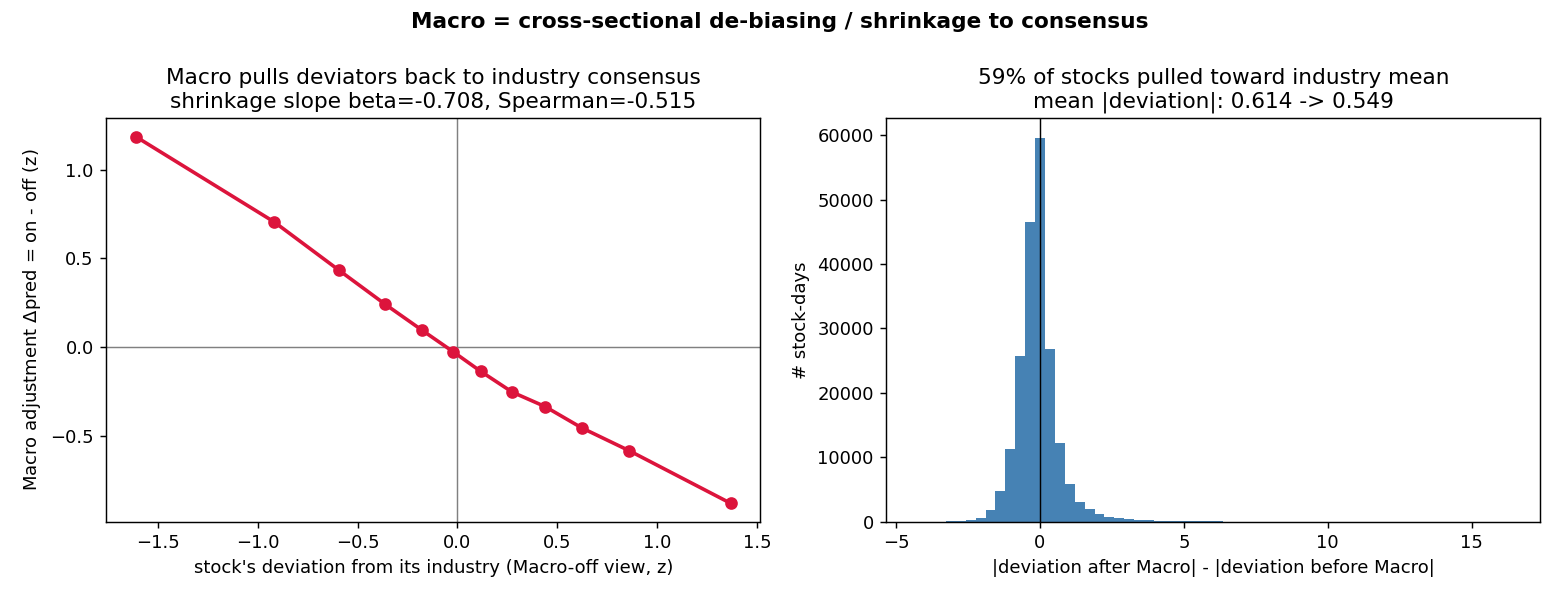
\includegraphics[width=\linewidth]{figures/macro_shrinkage.png}
\caption{开 / 关 Macro 的预测对比（baseline，测试期 2025-07 至 2026-05，约 $20$ 万个"股票-日"样本）。左图
横轴是个股相对其行业均值的偏离（关 Macro 时），纵轴是开 Macro 对该预测的调整量 $\Delta\text{pred}$：偏离越远
的票被往回拉得越狠（收缩斜率 $\beta=-0.708$，Spearman $\rho=-0.515$）。右图是全市场平均绝对偏离的分布对比，
$59\%$ 的票开 Macro 后更靠近行业均值，均值从 $0.614$ 降到 $0.549$。两图同指一件事：Macro 在系统性地把极端
预测往群体中心压。}
\label{fig:shrinkage}
\end{figure}

反事实收缩无法复现 Macro 的收益（图~\ref{fig:lambda}、表~\ref{tab:lambda}）：按式~\eqref{eq:lambda} 把关
Macro 的预测向行业均值收缩，两个种子的峰值（$+130\%$ / $+102\%$）都明显低于各自 base（$+166\%$ / $+129\%$），
也没有先升后降的甜区。向行业均值收缩替代不了 Macro，说明它调整预测时参照的不是行业均值。

\begin{figure}[H]
\centering
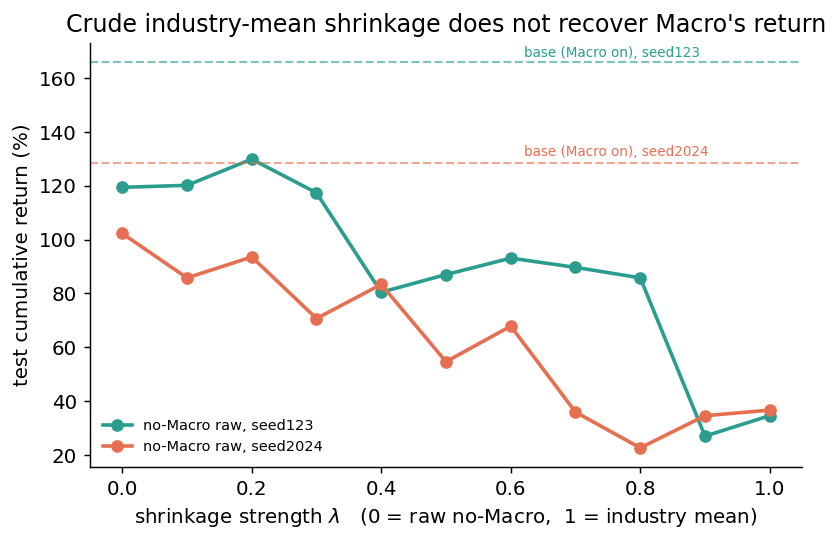
\includegraphics[width=0.66\linewidth]{figures/fig_lambda.png}
\caption{反事实实验：把关掉 Macro 的预测按强度 $\lambda$ 人工向行业均值收缩（$\lambda{=}0$ 不收缩，$\lambda{=}1$
完全收缩到行业均值），逐 $\lambda$ 回测，看"手工去偏"能否复现 Macro 的收益。两条实线是 seed 123 / 2024 的测试
累计收益，虚线是各自的 base（Macro 开）。所有 $\lambda$ 下实线都低于虚线、也没有先升后降的甜区——往行业均值
收替代不了 Macro。}
\label{fig:lambda}
\end{figure}

\begin{table}[H]
\centering
\caption{反事实实验的代表性取值（测试期累计收益 \%）。$\lambda$ 是人工向行业均值收缩的强度（$0{=}$ 不收缩，
即关 Macro 的原始预测；$1{=}$ 完全收缩到行业均值）；最右列 base 是 Macro 开启的真实收益。两个种子的峰值
（$\lambda{=}0.2$ 处 $129.9$、$\lambda{=}0$ 处 $102.3$）都明显低于 base（$166.0$、$128.6$），且整体随 $\lambda$
增大走低——把行业均值当替代品，无法复现 Macro 的收益。}
\label{tab:lambda}
\begin{tabular}{lccccc}
\toprule
& $\lambda{=}0$ & $\lambda{=}0.2$ & $\lambda{=}0.5$ & $\lambda{=}1$ & base(Macro on) \\
\midrule
seed123  & $+119.4$ & $+129.9$ & $+87.0$ & $+34.6$ & $+166.0$ \\
seed2024 & $+102.3$ & $+93.6$  & $+54.6$ & $+36.7$ & $+128.6$ \\
\bottomrule
\end{tabular}
\end{table}

真实参照落在注意力分布里。三层 Macro 的注意力软分组与申万行业标签的归一化互信息（NMI——信息论里衡量两个
分组重合度的指标，$0$ 为毫无关系、$1$ 为完全重合）都只有 $0.22\!\sim\!0.24$——远够不上还原行业（那要接近
$1$）；注意力本身高熵弥散，每只票平均覆盖当日约 $985$ 只里的 $877$ 只、Gini 约 $0.23$，不是按行业标签的稀疏
图；把注意力按行业聚合来看也是这样（图~\ref{fig:indagg}）——同业之间的平均注意力（对角）甚至比跨行业（非
对角）还略低（比值 $0.93$），真正亮的是几条被全市场共同关注的"枢纽行业"竖列，是一张广撒、跨行业的图，而非
行业块对角。那它锚的是不是"共动"？共动方向一致率给出全市场的答案，而且集中在\emph{第一层}：第一层 Macro 中，每只查询
股 top-$10$ 关注对象的当日同向率为 $61.7\%$，比"随机选 $10$ 只"的同日基线 $58.1\%$ 高出 $+3.6$pp（$208$ 个交易
日汇总，标准误仅 $0.4$pp、约 $9$ 倍标准误，统计上很稳，但幅度温和），且越靠前的关注对象这一超额越集中
（图~\ref{fig:codir}）。更深的两层不再高于随机（反而略低 $3\!\sim\!4$pp）——深层注意力作用在已被前层精炼过的
表征上，不再直接锚原始的当日涨跌。所以"按共动结构连接"主要是第一层的行为：它在每个交易日把查询股动态连向当天
\emph{倾向}同向波动的少数伙伴——这是一种\emph{轻微但稳定}的共动倾斜（$+3.6$pp、统计稳健但幅度小），而非强关系图。

\begin{figure}[htbp]
\centering
\begin{minipage}[b]{0.42\linewidth}\centering
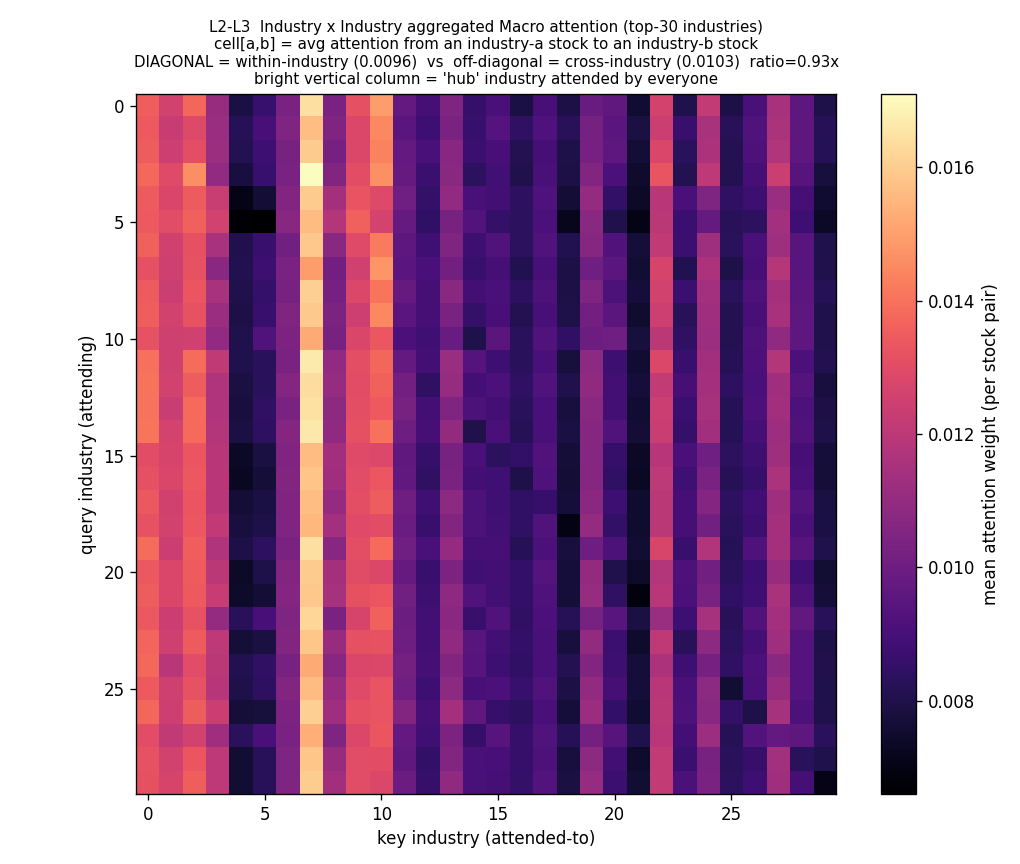
\includegraphics[width=\linewidth]{figures/macro_indagg.png}\\[3pt]
{\small (a) 注意力按行业聚合}
\end{minipage}\hfill
\begin{minipage}[b]{0.54\linewidth}\centering
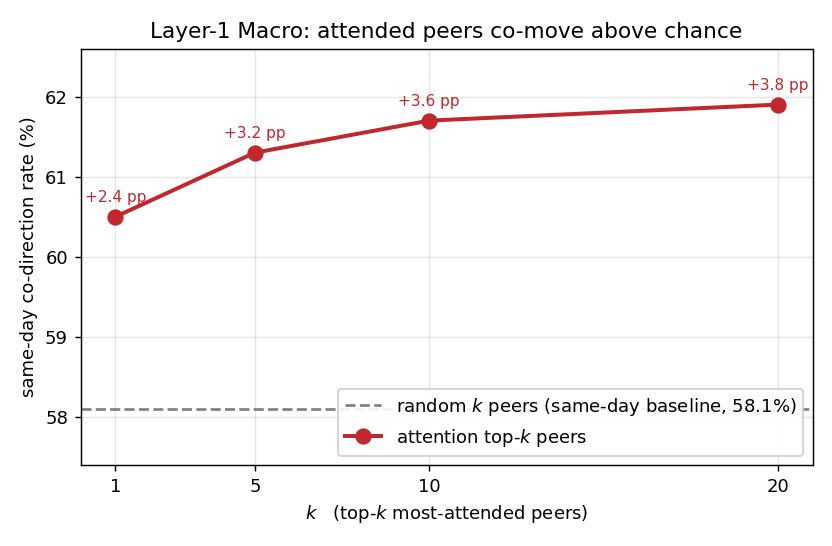
\includegraphics[width=\linewidth]{figures/macro_codir.png}\\[3pt]
{\small (b) 共动方向一致率}
\end{minipage}
\caption{Macro 收向的“池子”是什么。\textbf{(a)} 把注意力按申万行业聚合（前 $30$ 个行业，颜色为“一只行业-$a$ 的
股票分给一只行业-$b$ 的股票”的平均注意力）：对角（同业）平均 $0.0096$、反而略低于非对角（跨业）$0.0103$，比值
$0.93$——没有“同行业互相关注”的块对角，亮的是几条被全市场共同关注的“枢纽行业”竖列，是一张广撒、跨行业的图。
\textbf{(b)} 第一层 Macro 的 top-$k$ 关注对象当日涨跌同向率（全 $208$ 测试日、每日全市场），始终高于“随机选
$k$ 只”的同日基线 $58.1\%$ 约 $+2.4\!\sim\!3.8$pp——更偏向当天同向波动的伙伴，但超额幅度温和。}
\label{fig:indagg}
\label{fig:codir}
\end{figure}

case study 则从另一面印证"非行业"：权重最高的少数关注对象，多是\emph{跨}申万行业、却有真实题材 / 产业链联系
的个股（图~\ref{fig:casestudy}）。科技板块的宏发股份，关注簇是一条跨行业的 AI 硬件链（光芯片源杰 $\to$ 光器件
天孚 $\to$ 光模块中际旭创 / 新易盛，外加 PCB 胜宏 / 生益、电力侧思源 / 金盘）；有色板块的神火股份，关注簇是
电解铝同行集群（天山铝业、宏桥、云铝、中孚，加铜业江西铜业）。逐一查证见附录~\ref{sec:casestudy-rel}。

\begin{figure}[H]
\centering
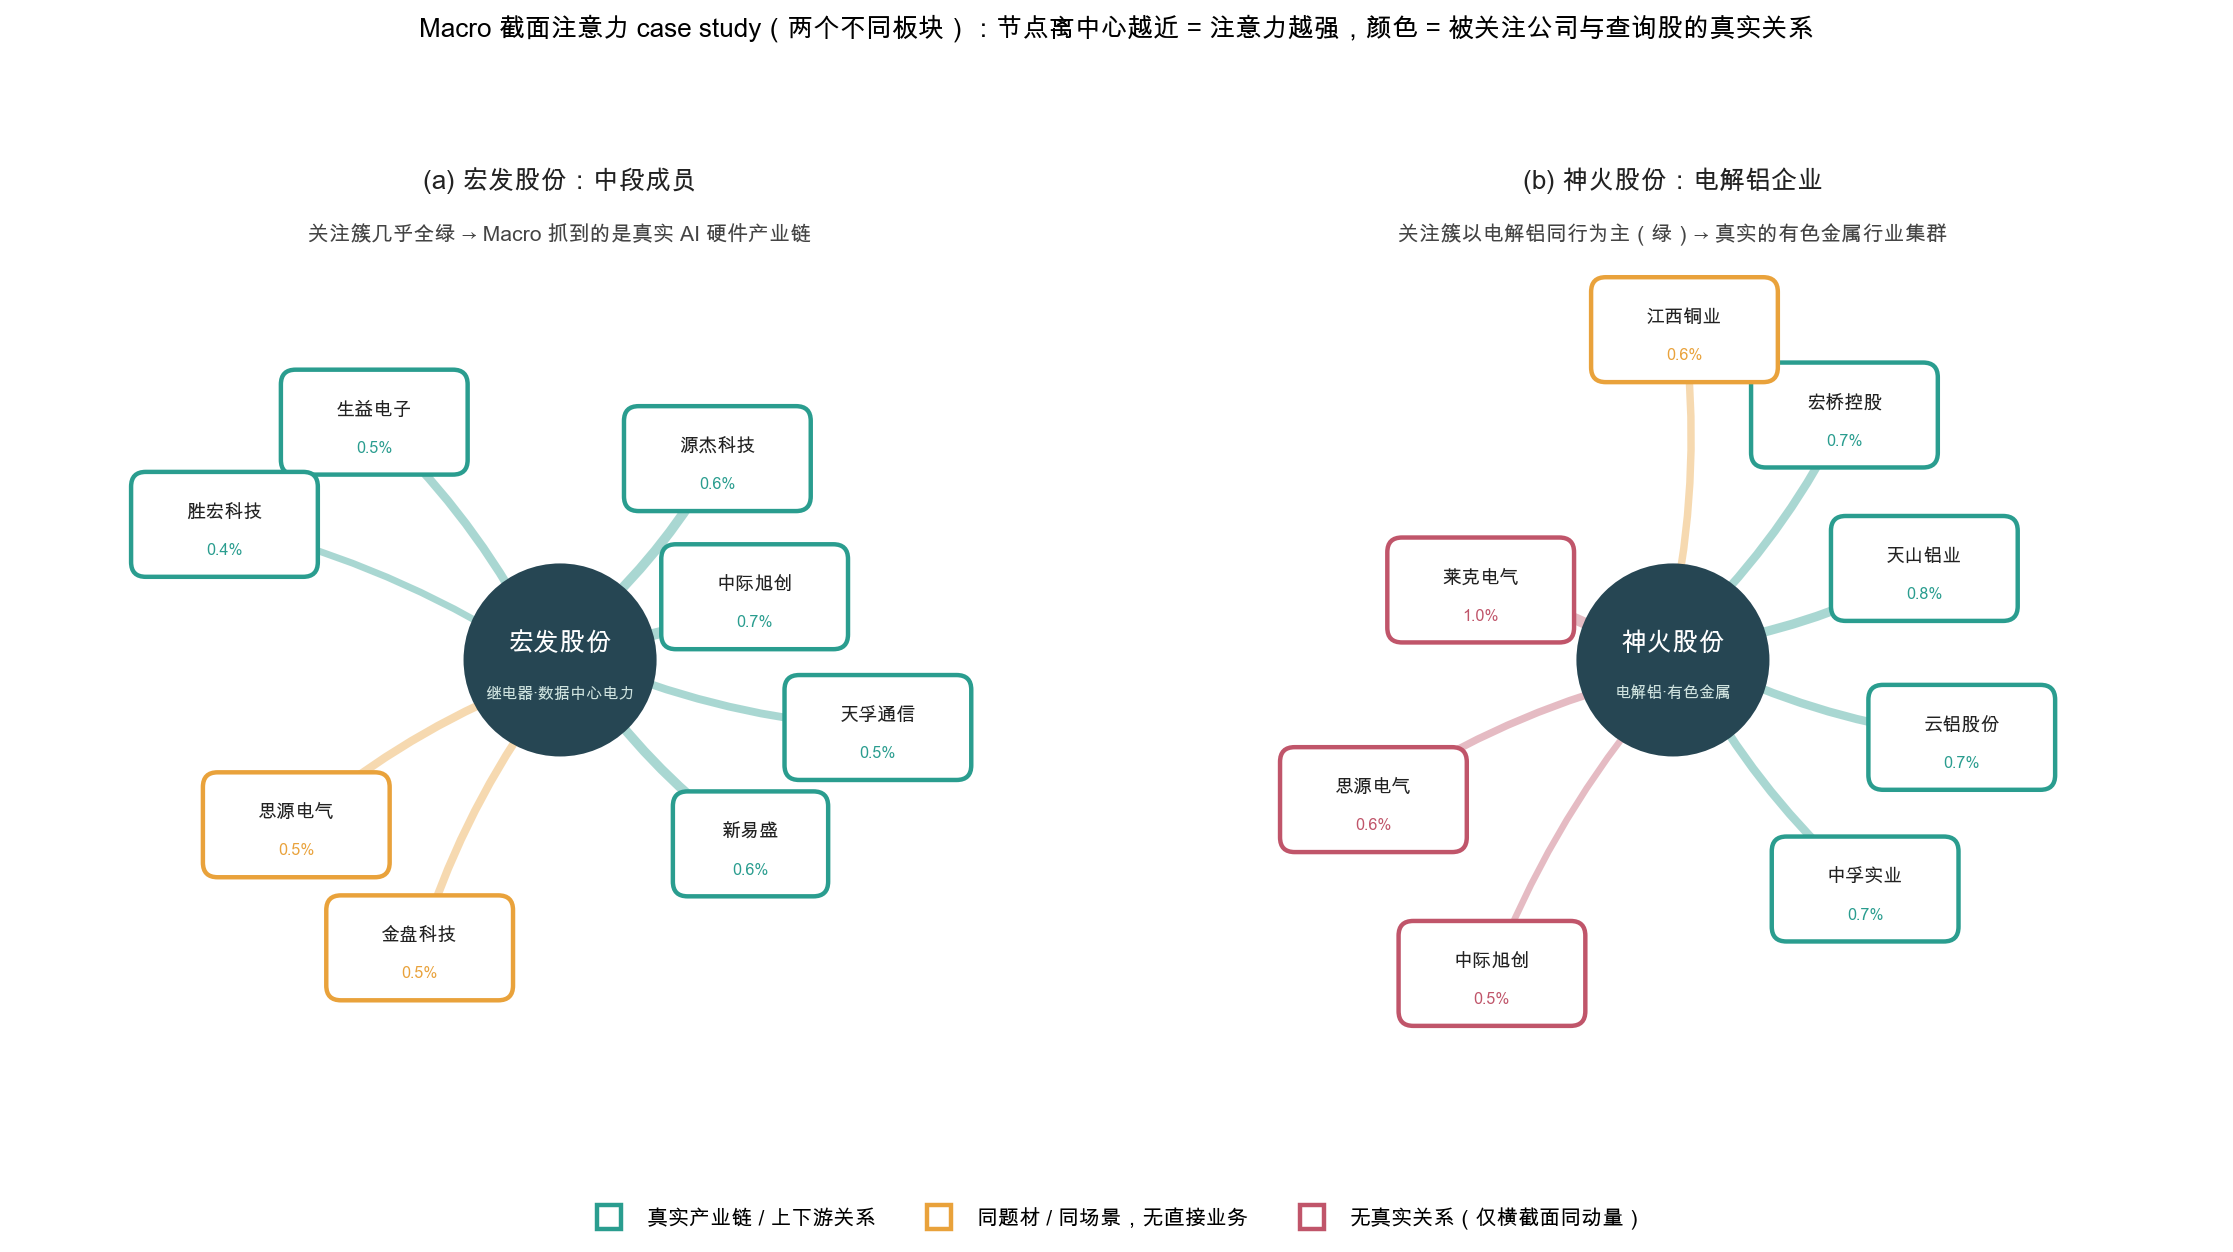
\includegraphics[width=0.96\linewidth]{figures/macro_casestudy.png}
\caption{Macro 截面注意力的可视化（baseline，交易日 2025-12-11）。每张图是一只查询股（中心节点）与其权重
最高的关注对象：节点离中心越近表示注意力越强；颜色标注被关注公司与查询股的\emph{真实}关系（绿 $=$ 真实产业
链 / 同行业，橙 $=$ 同题材 / 同场景但无直接业务，红 $=$ 无真实关系、仅横截面同动量）。(a) 宏发股份（科技板块，
继电器）：强关注落在一条\emph{跨}行业的真实 AI 硬件链上（光芯片源杰 $\to$ 光器件天孚 $\to$ 光模块中际旭创 /
新易盛，外加 PCB 胜宏 / 生益、电力侧思源 / 金盘）。(b) 神火股份（有色板块，电解铝）：强关注锁定\emph{同}行业
集群（天山铝业、宏桥、云铝、中孚，加铜业江西铜业）。两例分属不同板块、关系形态不同，强关注却都是真实的共涨
共跌同伴——Macro 按截面共动结构聚合，而非按行业标签（少数红色为同动量噪声，如莱克电气）。}
\label{fig:casestudy}
\end{figure}

\textbf{\heiti 分析.} 四组测量拼到一起，共同指向同一个\emph{目前最自洽的}机制解释：Macro 像一个学出来的截面
去噪器。它把每只票的分数往同伴共识上收（图~\ref{fig:shrinkage} 的去偏）；这个共识不是静态的行业均值——手工往
行业均值收复现不了它的收益（图~\ref{fig:lambda}），注意力分组与行业的 NMI 只有 $0.23$、按行业聚合还略偏跨行业
（图~\ref{fig:indagg}）；而它收向的同伴当天确有\emph{共动结构}——第一层关注对象的同向率显著高于随机
（图~\ref{fig:codir}），case study 里那些跨行业的强关注也对得上人工查证的题材 / 产业链（图~\ref{fig:casestudy}）。
需强调：图~\ref{fig:codir} 说明的是被关注伙伴存在\emph{当日共动结构}（关注对象非随机），\emph{并不}证明这些同伴
携带真实 alpha——"借同伴去噪是否真换来更稳的排序"由双轴消融关 Macro 的 $-46$pp（§\ref{sec:pillars}）旁证，而非由
共动率本身证明。

它为什么能换成收益，落点还是在噪声上。低信噪比下，单股打分方差大、个体信号不可靠；把每只票的估计往一池相关
同伴一收，特异噪声被平均掉，\emph{按 James--Stein / 经验贝叶斯框架估计方差应当下降}——这是"用一点偏差换大量
方差"的框架性预期（须重申：本文未直接测得方差降幅，§\ref{sec:macro} 理论段已声明，这里是框架推断而非实测），
而它恰好在噪声最大时最划算。这一框架也自洽地解释了两件本来像"缺点"的事：注意力为什么那么弥散（每票平均覆盖
$877/985$）、共动为什么只是温和的 $+3.6$pp——按该框架，一个好的去噪池本就该\emph{广撒}（撒得越广、方差应降
得越多）、只带\emph{轻微}的相关倾斜（够把无关股票的偏差压住即可）。弥散加弱共动不是没找到结构，而更像一个
偏差-方差权衡合理的去噪器该有的样子。

还有一点值得点明：没有任何一行监督让 Macro 去找同涨同跌的股票，训练目标里只有截面排序。"关注当天和自己一起
动的伙伴"是模型\emph{自发学到}的——因为借相关同伴去噪，能把排序排得更稳。共动是\emph{手段}、排序准确才是
\emph{目的}，这条手段并非显式指定，而是在低信噪比下自行涌现。比起 RSR、超图那类要从外部喂进一张股票关系图的
做法，这里的关系图是模型按当日共动自行（且较弱地）形成的；深层则在前层精炼过的表征上继续加工。

这套刻画也有边界。"去噪有效"这条因果链，目前是几组证据共同指向的最自洽解释，还没有直接测到"方差到底降了多少、
收益正好来自这里"；共动信号本身不强、且只在第一层清晰；对动量最极端的龙头（如全年 $+424\%$ 的新易盛），关注
簇会退化成"跨题材的强趋势拼盘"，模型也分不太清真实产业趋势与短期概念炒作（如改名追逐量子概念的联美控股）。


% ================================================================ 5 讨论
\section{讨论与局限}\label{sec:discuss}
\textbf{\heiti 选点与方差是被低估的一等问题.} 本文最可迁移的教训是：在低信噪比的截面选股上，"怎么训练、
怎么选检查点"对最终收益的影响，往往大于"用什么架构"。验证 IC 与样本外收益反向（第~\ref{sec:select} 节）、
同一配置跨种子从 $-3\%$ 到 $+117\%$ 的波动，都说明单次运行报告的"提升"很可能落在噪声带内。这要求评测协议
本身做文章——最优 ckpt 衡量能力上限、验证选点衡量可部署性、多种子衡量稳定性，缺一不可。

\textbf{\heiti best-ckpt 是上界，不是可部署值.} 本文用最优 ckpt 作为"能力天花板"以剥离选点方差，但它按
测试收益挑点，是 oracle 上界；真正可部署的是验证段选点。报告同时给出两者，避免把上界误读为实盘表现。
如何在不偷看测试集的前提下稳健选点（多检查点集成、或验证 IC 之外的稳定性指标），是一条值得继续的方向。

\textbf{\heiti 市场共模信息的天花板.} 截面排序的目标会在很大程度上抵消对所有股票影响相近的\emph{共模}
市场信号：当所有股票被同一市场行情同向推动时，它们的相对次序几乎不变，而本文优化与评测的都是相对次序。
因此\emph{共模}市场信息对截面 alpha 的增量天然有限，这也是本文默认只用少量市场指数、且不依赖复杂市场调制结构的原因。
\textbf{\heiti 须与 Macro 区分：} 这里说"增量有限"的是\emph{共模}（market-wide common mode，被截面排序抵消的那部分），
而 Macro 之所以是支柱（关掉 $-46$pp，§\ref{sec:pillars}/\ref{sec:macro}）靠的\emph{不}是共模，而是\emph{个股之间的相对
结构}——把每只票往一群相关同伴的共识上收、去掉个股特异噪声。共模是被抵消的背景，相对结构才是 Macro 吃的信号，
两者并不矛盾。

\textbf{\heiti 方法比收益数字更立得住.} \msqa{} 在统一口径下收益高于所有重现的 baseline，但收益数字不是
本文的落点——它依赖种子与选点、在方差红线下波动很大。真正立得住的是方法：每根轴都能单独关掉，支柱作用
因此可以直接验证（第~\ref{sec:pillars} 节）；注意力权重能钩出来，Macro 在关注谁因此可以被归因
（第~\ref{sec:macro} 节）；每个结论都压在 $\pm60$pp 红线下，真实效应和噪声因此能分开。

\textbf{\heiti 局限.} (i) 测试窗口较短，金融数据噪声大，绝对收益的统计置信度有限；(ii) 训练用
沪深 300、回测用 top1000，两者口径不完全一致；(iii) 部分配置（尤其个别种子）保存的检查点较稀疏，最优 ckpt
是"现有检查点中的最优"而非连续意义上的最优；(iv) 未使用新闻 / 舆情等外部文本数据——这类信息部分以情绪、
事件形式作用于价格、与前文"市场共模信息的天花板"相关，且公开时往往已带滞后，本文特征只用量价 $+$ 基本面 $+$ 资金流。

% ================================================================ 6 结论
\section{结论}\label{sec:conclusion}
本文围绕 A 股截面选股，给出\textbf{两个模型设计创新}：其一，把双轴（时间轴 Micro $+$ 截面轴 Macro）交互重构为
一个解耦、可堆叠、可逐轴关断的特征提取原语 \msq{} Block，多层堆叠让两轴迭代重读；其二，全程保留 $(S,T,D)$
表征、采用因果时序、对每个时间步施加密集的截面排序监督。在统一评测协议（最优 ckpt $+$ 多种子 $+$ 方差红线）下，
穿过红线仍然成立的稳健结论可归为\textbf{三点发现}。\emph{（一）两个设计都经消融证实有效}：双轴缺一皆显著掉收益
（误差带与 base 不重叠）、堆叠带来可见的迭代增益，密集监督也显著优于只监督末步（两口径误差带均不重叠，
§\ref{sec:abl-dense}）。\emph{（二）Macro 的最自洽机制解释是截面去噪器}：把每只股票的预测往一群数据驱动的相关
同伴共识上收、压低单股噪声（软分组与申万行业互信息仅 $0.23$，不是行业均值、也不是外部关系图），低信噪比正是
这种去噪有效的前提——但这是目前证据下的最自洽\emph{解释}、非因果证明。\emph{（三）验证 IC 与样本外收益反向}，
标准选点准则会系统性选到泛化更差的模型，凸显评测协议之必要。

贯穿全文的判断是：低信噪比下，怎么训练、怎么选点，比架构长什么样更决定成败。\msqa{} 的收益高于所有
重现的 baseline，但它真正的立足点是方法——双轴可以逐轴关断来定位支柱、注意力可以钩出来归因、每个结论都
压在 $\pm60$pp 红线下判真伪。后续工作可循着局限展开：(1) 不偷看测试集的稳健选点（针对选点失效）；(2) 在更长
测试窗口、统一训练 / 回测股票池口径下复核绝对收益（针对局限 i/ii）；(3) 用时间池化对照补测"保留时间维"本身的
贡献，即密集监督消融未覆盖的\emph{表征设计}那一半（§\ref{sec:abl-dense}）；(4) 直接测量 Macro 带来的预测方差
下降，以把去噪从"最自洽解释"推进到因果验证；(5) 同参数量下"宽单层 vs 堆叠"的决定性对照、并把可解释性结论
反哺成架构改进再验证。

% ================================================================ 亮点与思考
\section*{实验亮点}
\begin{itemize}
  \item 把双轴交互做成一个可逐轴关断的 \msq{} Block——每根轴都能单独撤掉重测，支柱作用因此可以直接证伪，
        而不是只靠叙述。
  \item 一套把真实效应与噪声分开的评测协议：最优 ckpt 衡量能力上界、验证选点衡量可部署性、多种子定方差，
        并以 $\pm60$pp 红线判真伪。这是本项目最可迁移的产出。
  \item 为 Macro 给出一个可证伪、且目前证据下最自洽的机制解释——它\emph{表现得像}一个学出来的截面去噪器：
        NMI 仅 $0.23$、$\lambda$ 扫描否定行业均值替代，排除了"锚是行业"；全市场共动检验则量到第一层关注对象
        确有当日共动结构（温和但显著，注意这是共动、非真实 alpha）。但尚未直接测得方差下降的因果证据，故是\emph{解释}
        而非证明；可解释性没有停在叙述。
  \item 两个反直觉发现：验证 IC 与样本外收益反向（$-0.75$）；固定模型信号、只改交易策略，收益能差
        $130$pp，与架构改动同量级。
\end{itemize}

% ================================================================ 附录
\appendix

本附录给出正文未展开的输入特征、消融与诊断细节，口径与正文一致（最优 ckpt、多种子 seed 42/123/2024、$\pm60$pp 红线）。把它们
放在一起看有一个统一的意义：正文报的收益不依赖某个精心调出的超参。除少数会触发崩溃的设计（二分类标签、
过短的时间窗、同时去掉因果与高斯）外，注意力头数、子层顺序、近邻带宽、稀疏化、换手正则等改动的多种子收益
都落在 base（$+155\pm19$）的红线带内，与噪声不可区分。汇总见表~\ref{tab:appendix}。

\section{输入特征：35 个量价 / 基本面 / 资金流因子}\label{sec:features}
所有特征均按个股时间序列计算（\texttt{groupby(ts\_code)}，绝不跨股票）、统一以 \texttt{f\_} 前缀标识，
不在全局做标准化、交由后续 rolling 标准化以防泄漏。baseline 默认使用 35 个因子，分 7 组（表~\ref{tab:features}）：
价量技术类（前五组，共 27 个）取自 Qlib 的 Alpha158 因子库~\cite{qlib} 的子集；基本面 6 个直接取自 Tushare
\texttt{daily\_basic} 字段；资金流向 2 个为自行构造（完整公式见下）。更大的因子档（\texttt{medium}$\approx 80$、
\texttt{full}$\approx 158$，后者为完整 Alpha158 子集）用于因子数量的扩展实验。

\begin{table}[H]
\centering\small
\caption{baseline 输入的 35 个因子（\texttt{feature\_set=basic}）。来源标注：A=Alpha158 子集~\cite{qlib}、
D=Tushare \texttt{daily\_basic}、S=自行构造。$O/H/L/C/V$ 为开/高/低/收/量，$r_1=C_t/C_{t-1}-1$，
$\mathrm{MA}_k/\mathrm{VMA}_k$ 为 $k$ 日均值，$\mathrm{std}_k$ 为 $k$ 日滚动标准差。}
\label{tab:features}
\begin{tabular}{@{}p{1.9cm}p{6.0cm}cp{3.4cm}@{}}
\toprule
组（来源） & 因子 & 数 & 定义 \\
\midrule
多尺度动量 (A) & \texttt{f\_ret\_k}, $k\in\{1,2,3,5,10,20,30,60\}$ & 8 & $C_t/C_{t-k}-1$ \\
均线偏离 (A) & \texttt{f\_close\_ma\_k}, $k\in\{5,10,20,30,60\}$ & 5 & $C_t/\mathrm{MA}_k-1$ \\
波动率 (A) & \texttt{f\_vol\_k}, $k\in\{5,10,20,30,60\}$ & 5 & $\mathrm{std}_k(r_1)$ \\
K线形态 (A) & \texttt{f\_kmid}, \texttt{f\_klen}, \texttt{f\_kup}, \texttt{f\_klow} & 4 & 见下式 \\
成交量 (A) & \texttt{f\_vol\_ratio\_k} $(k{\in}\{5,10,20\})$；\texttt{f\_vol\_chg\_1}；\texttt{f\_amount\_chg\_1} & 5 & $V_t/\mathrm{VMA}_k$；量、额的 1 日变化率 \\
基本面 (D) & \texttt{f\_turnover\_rate}, \texttt{f\_turnover\_rate\_f}, \texttt{f\_volume\_ratio}, \texttt{f\_pe\_ttm}, \texttt{f\_pb}, \texttt{f\_ps\_ttm} & 6 & 换手率 / 自由流通换手 / 量比 / PE / PB / PS（直接取字段） \\
资金流向 (S) & \texttt{f\_mf\_net\_ratio}, \texttt{f\_mf\_big\_small\_diff} & 2 & 见下式 \\
\midrule
\multicolumn{2}{@{}l}{合计} & 35 & \\
\bottomrule
\end{tabular}
\end{table}

\noindent\textbf{\heiti K 线形态（沿用 Alpha158 定义）.} 设开 / 高 / 低 / 收为 $O,H,L,C$：
\[
\texttt{f\_kmid}=\frac{C-O}{O},\quad \texttt{f\_klen}=\frac{H-L}{O},\quad
\texttt{f\_kup}=\frac{H-\max(O,C)}{O},\quad \texttt{f\_klow}=\frac{\min(O,C)-L}{O}.
\]

\noindent\textbf{\heiti 自构资金流因子（完整公式）.} 记当日成交额 $A$（千元）、当日净流入额 $M$（万元，
Tushare \texttt{net\_mf\_amount}）、大 / 特大 / 小单买入额 $B_{lg},B_{elg},B_{sm}$（万元）：
\begin{align*}
\text{\texttt{f\_mf\_net\_ratio}} &= \mathrm{clip}\!\Big(\frac{M\times 10^{4}}{A\times 10^{3}},\ -5,\ 5\Big)
= \mathrm{clip}\!\big(10M/A,\,-5,\,5\big),\\[3pt]
\text{\texttt{f\_mf\_big\_small\_diff}} &= \frac{(B_{lg}+B_{elg})-B_{sm}}{(B_{lg}+B_{elg})+B_{sm}+1}.
\end{align*}
这两个是 baseline 35 维里仅有的两个非 Alpha158 因子，专为 A 股补一个量价之外的\emph{资金面}维度——A 股散户
主导、价格常被资金与情绪推着走（§\ref{sec:intro}），Tushare 的 \texttt{moneyflow} 恰好提供了 Alpha158 没有的
资金结构信息。下面解释它们各自的含义与作用。

\textbf{\heiti （1）\texttt{f\_mf\_net\_ratio}：净流入强度.} 把当日\emph{净流入额}除以\emph{成交额}（量纲统一到
元后裁剪到 $[-5,5]$；换算系数 $10$ 来自 Tushare 成交额记千元、资金流记万元）。它衡量"这只票今天的成交里有多大
比例是净买入推动的"：$>0$ 为资金净流入（买盘主导、可能在吸筹）、$<0$ 为净流出。之所以\emph{除以成交额}而非
直接用净流入额，是因为个股成交规模相差几个数量级、绝对额无法横向比较；归一成比率后，这个"资金面强弱"信号才
能放进当日截面里跨股票排序——正契合本文截面选股的目标。裁剪 $[-5,5]$ 是为压住停复牌、单日异动带来的极端值。

\textbf{\heiti （2）\texttt{f\_mf\_big\_small\_diff}：主力—散户买盘结构.} 用 $(\text{大单}+\text{特大单买入})-
\text{小单买入}$ 再除以三者之和（分母 $+1$ 防零除），归一到 $[-1,1]$ 区间。在 A 股，大 / 特大单通常对应机构或
游资（"主力"），小单对应散户，故该因子刻画的是\emph{谁在买}：$>0$ 表示主力买盘强于散户（主力进场），$<0$ 表示
更多由散户接盘、主力可能在派发。在散户主导、情绪驱动的市场里，"谁在买"往往比"买了多少"更有信息含量——主力
净买入的个股后续相对强势的概率更高；这正是量价、估值之外，从资金\emph{结构}维度补上的一个截面可比信号。

\section{架构消融}\label{sec:abl-arch}
这一组检验正文的收益是否依赖某个架构超参的特定取值。逐一改动后回测，下面几项都落在 base（$+155\pm19$）的
红线带内，只有最后一项例外。

\textbf{\heiti 注意力头数.} 头数决定模型能并行追踪几种关系模式，是最常被调的超参。Micro（时间轴）头数从默认
$4$ 改成 $2$ / $8$，得 $+186\pm37$ / $+163\pm27$；Macro（截面）头数从默认 $2$ 改成 $1$ / $4$，得 $+161\pm26$ /
$+165\pm33$。四档全与 base 重叠，收益对头数不敏感。

\textbf{\heiti 子层顺序.} 每个 Block 默认先 Micro 后 Macro。反过来先截面后时序，得 $+142\pm20$，与 base 重叠
——两轴谁先谁后不改变结果，因为多层堆叠后两者本就反复交替。

\textbf{\heiti 稀疏 Macro.} 截面注意力默认连全市场。若每只股票只关注打分最高的 $30$ 只邻居，得 $+161$（两
种子，与 base 同量级、尚待第三种子确认），不劣于全连接。这与 §\ref{sec:macro} 一致：Macro 要的是少数稳健的
共识锚点，长尾的稠密连接是可省的噪声。

\textbf{\heiti 多尺度 Micro.} 让堆叠的不同层用不同回看长度（自底向上 $8/5/3$ 天）以兼顾多个时间尺度，得
$+162\pm30$，与单一尺度的 base 重叠——多尺度没带来额外收益。

\textbf{\heiti 宽度.} 加宽表示维度 $D$（$64/128/256$，最优-ckpt 三种子）：$+79\pm19\%$ / $+155\pm19\%$ /
$+154\pm17\%$。$D{=}64\to128$ 收益补齐到 base 一线，但 $128\to256$ 再翻一倍参数却走平（$155\to154$，落在误差带
内）——加宽到 base 宽度即饱和。这与堆叠深度恰成对照（$L{:}3\to4\to5$ 仍从 $155$ 抬到 $187$、$201$）：同样往
base 上堆参数，加在宽度上饱和、加在深度上还涨，佐证深度增益来自迭代重读而非纯参数量（详见 §\ref{sec:depth}）。

\textbf{\heiti 去因果 / 全局注意力.} 前面都是"改了也没事"，这一项是反例。同时去掉 Micro 的因果掩码（改双向）
与高斯先验，时间轴注意力退化成无约束的全局注意力，得 $+52$（\emph{seed42 单种子}）。须按本文判据谨慎：单种子
不足以精确定位，但其相对 base（$+155$）的降幅约 $103$pp、达 $\pm60$pp 红线的近两倍，远超种子噪声量级，故"完全
放开会显著变差"这个\emph{方向}应是稳健的（精确幅度与多种子确认留待后续）。这说明"只看过去、且偏好近邻"这层
时序归纳偏置确有价值，是少数方向稳定的负向改动之一。

\subsection{Micro 的近邻先验：高斯带宽与时间窗}\label{sec:abl-micro}
Micro 在时间轴自注意力上叠加了一个随时间距离衰减的高斯先验（§\ref{sec:m-block}），由两个旋钮控制，这里
逐一消融。\textbf{\heiti 高斯带宽 $\sigma$} 控制"偏好近邻"的强弱：$\sigma{=}2/4/8$ 分别得 $+139$ / $155$ /
$+112$，三档都与 base 重叠，带宽并不敏感。\textbf{\heiti 完全去掉高斯先验} 得 $+169\pm34$（三种子），同样
落在噪声带内——\emph{加不加}这个先验都没有显著差异，它更像一个无害的归纳偏置而非收益来源。\textbf{\heiti
时间窗 $\tau$}（每个时间步最多回看几天）则有明确的下界：$\tau{=}1$（只看前一日）收益崩溃到 $+33\pm14$，而
$\tau\ge3$ 后即回到与 base 同一量级（$\tau{=}3/5/8/15$ 约 $+135/+134/+155/+152$）。可见 Micro 确实依赖近邻
加权，但只要窗口不过短，具体长度并不敏感。

\section{训练与正则}\label{sec:abl-train}
训练侧附加实验——对抗训练（FGSM 扰动 $\varepsilon{=}0.1$，$+181\pm14$）与换手正则（在训练
目标里惩罚换手，$\lambda{=}0.1$，$+139\pm72$）——均未稳定越过方差红线，两者的多
种子收益同样落在 base 红线带内。训练目标本身（回归 / 排序 / 分类）的系统对照见 §\ref{sec:objective}。

\begin{table}[H]
\centering
\caption{附录消融汇总（test 累计收益，最优-ckpt 多种子）。base $=+155\pm19$；除注明外为种子 123/2024。}
\label{tab:appendix}
\begin{tabular}{lcc}
\toprule
消融 & 收益（mean$\pm$std） & 判读 \\
\midrule
Micro 头数（$2$ / $8$，默认 $4$）   & $+186$ / $+163$ & 与 base 重叠 \\
Macro 头数（$1$ / $4$，默认 $2$）   & $+161$ / $+165$ & 与 base 重叠 \\
子层顺序（先 Macro 后 Micro）       & $+142\pm20$    & 与 base 重叠 \\
稀疏 Macro（每股 attend top-$30$）  & $+161$         & 不劣于全连接 \\
多尺度 Micro（回看 $8/5/3$ 天）     & $+162\pm30$    & 与 base 重叠 \\
高斯带宽（$\sigma{=}2/4/8$）        & $+139$ / $155$ / $+112$ & $\sigma$ 不敏感 \\
去高斯（$\sigma\to0$，三种子）      & $+169\pm34$    & 与 base 重叠 \\
时间窗（$\tau{=}1/3/5/8/15$）       & $+33$/$135$/$134$/$155$/$152$ & $\tau{=}1$ 崩；$\tau\ge3$ 同量级 \\
对抗训练（$\varepsilon{=}0.1$，三种子）& $+181\pm14$  & 红线内 \\
换手正则（$\lambda{=}0.1$，三种子） & $+139\pm72$    & 红线内 \\
去因果 $+$ 去高斯（全局注意力）     & $+52$（seed42） & 跌出红线（单种子，方向稳健） \\
\bottomrule
\end{tabular}
\end{table}

\subsection{训练配方：学习率、优化器与调度器}\label{sec:abl-recipe}
上一节（表~\ref{tab:appendix}）在最优-ckpt 口径下考察了\emph{架构与正则}旁路；这里转向\emph{训练配方}本身——
学习率、优化器、学习率调度与 dropout 四个旋钮，并刻意改用\textbf{\heiti 可部署的"验证选点 $\times$ 3 种子"口径}
（§\ref{sec:select}）来报告。原因是：训练配方的改动会直接左右"何时收敛、验证集挑中哪个 ckpt"，因此最该在
这个会暴露选点与种子方差的口径下检验，看哪些选择能扛过 $\pm60$pp 的噪声。本表回测引擎为简化的 TopK 组合
（top1000 池、开盘成交），与正文主表的机构化策略不同，故\emph{只做表内相对比较}。

\begin{table}[H]
\centering
\caption{训练配方消融：test 累计收益，验证选点 $\times$ 3 种子，简化 TopK 回测引擎（top1000 / 开盘成交）。
默认 base $=$ AdamW、lr $10^{-5}$、无调度器、dropout $0.1$，同口径参照 $+67\%$（seed 42）。SGD 系已按惯例
放大学习率（动量 / Nesterov $10^{-3}$、Adagrad $10^{-2}$）。}
\label{tab:recipe}
\begin{tabular}{llcl}
\toprule
旋钮 & 配置 & 收益（mean$\pm$std） & 判读 \\
\midrule
学习率   & $10^{-4}$（偏高）       & $+41\pm25$           & \\
         & $5\times10^{-5}$       & $\mathbf{+107\pm48}$ & 甜区 \\
         & $10^{-6}$（偏低）       & $+33\pm15$           & \\
\midrule
优化器   & SGD$+$Nesterov         & $-5\pm3$    & \\
         & SGD$+$Momentum         & $-1.5\pm3$  & 全面、稳定地 \\
         & RMSprop                & $+14\pm19$  & 劣于 AdamW base \\
         & Adagrad                & $+33\pm16$  & \\
\midrule
调度器   & $+$cosine              & $+89\pm82$  & \\
         & $+$cosine\,warmup      & $+99\pm82$  & 均值偏高但 \\
         & $+$step                & $+97\pm97$  & 淹没于种子噪声 \\
\midrule
dropout  & $0$                    & $+35\pm26$  & \\
         & $0.2$                  & $+94\pm55$  & 与 base 重叠 \\
\bottomrule
\end{tabular}
\end{table}

三点结论。\textbf{\heiti（1）优化器是唯一跨种子稳健的硬约束。} 即便按惯例把 SGD 系的学习率放大 $100$–$1000$ 倍
（动量 / Nesterov 用 $10^{-3}$、Adagrad 用 $10^{-2}$，相对 AdamW 的 $10^{-5}$），它们的三种子收益仍紧贴 $0$
（Nesterov $-5\pm3$、SGD$+$Momentum $-1.5\pm3$，方差仅 $3$pp），而\emph{所有}基于 AdamW 的配置——base 及全部
学习率 / 调度器 / dropout 变体——都明显更高。这是少数方差远小于红线、且在每个种子上都成立的真实结论：稀疏、
高噪的截面梯度需要自适应步长。\textbf{\heiti（2）学习率存在甜区。} AdamW 内部 $5\times10^{-5}$（$+107$）优于
$10^{-4}$（$+41$）与 $10^{-6}$（$+33$），过高过低都伤；base 选的 $10^{-5}$ 略偏保守。\textbf{\heiti（3）调度器与
dropout 基本被种子噪声淹没。} 三种调度器的均值（$+89\sim99$）看似都高于 base，但 std 高达 $80$–$97$pp——其中
step 调度器在 seed 42 给出唬人的 $+186\%$，换 seed 2024 却是 $-7\%$。这恰是 §\ref{sec:select} 所述"选点 $\times$
种子"陷阱的活体样本：单一种子足以把一个纯噪声的旋钮包装成"最佳实践"，三种子一摊开便原形毕露。

\section{Macro 诊断图的统计构造}\label{sec:macro-prov}
正文 §\ref{sec:macro} 的四组 Macro 诊断图，其数据如何从原始预测 / 注意力一步步算到最终图表（样本单位、聚合方式、
统计量与随机基线的定义），统一汇总在表~\ref{tab:macro-prov}，便于复现与判读；这里的"构造"指统计定义，而非绘图所
用的软件工具。

\begin{table}[H]
\centering
\caption{Macro 诊断图的数据构造（provenance）。所有预测来自同一组 base 模型（seed 42/123/2024）的
Macro-on / Macro-off 两次推理，测试期 2025-07 至 2026-05，回测口径同 §\ref{sec:setup}。}
\label{tab:macro-prov}
\begin{tabularx}{\linewidth}{l>{\raggedright\arraybackslash}X>{\raggedright\arraybackslash}X}
\toprule
图 & 样本单位 / 输入 & 计算与统计量 \\
\midrule
图~\ref{fig:shrinkage}（收缩） & 全部"股票-日"（$\sim$20 万）；on/off 预测各逐日截面 $z$-score &
$\Delta\text{pred}{=}\hat r^{\mathrm{on}}{-}\hat r^{\mathrm{off}}$ 对"相对行业均值偏离"做 OLS 一次拟合
（$\beta$，\emph{未} winsorize，仅去非有限值）与 Spearman $\rho$；行业均值用 Macro-\emph{off} 的 $z$ 值算；
拉回比例与平均绝对偏离在 stock-day 上 pooled \\
图~\ref{fig:lambda}（反事实） & 行业内（每日 $\times$ 每行业）的 Macro-off 预测均值 &
按式~\eqref{eq:lambda} 逐 $\lambda\in\{0,0.1,\dots,1\}$ 向行业均值收缩后回测，得逐 $\lambda$ 测试累计收益
（结果文件 \texttt{lambda\_shrink.csv}）；仅 seed 123/2024（结果文件未含 seed42）；与 Macro-on 的 base 对比 \\
图~\ref{fig:indagg}（行业聚合 / NMI） & $A_{\mathrm{off}}$（末层，多头平均，去对角） &
行业$\times$行业格子 $=$ 行业 $a$ 的股票流向行业 $b$ 的平均注意力；NMI 为 $A_{\mathrm{off}}$ 对称化后
谱聚类（$k{=}\min(12,\#\text{行业})$）的簇与申万行业标签的归一化互信息；另做 200 次行业标签置换检验 \\
图~\ref{fig:codir}（共动方向） & 每交易日 $\times$ 每查询股，$A_{\mathrm{off}}$ 的 top-$k$ 关注对象（$k{\in}\{1,5,10,20\}$） &
同向 $=$ 当日涨跌 sign 一致比例；随机基线为当日同向的解析期望 $p^2{+}(1{-}p)^2$（结果文件 \texttt{rand\_agree} 列，
经数值核验，已扣大盘普涨跌）；"超出随机"的差额\emph{按交易日}聚合（$n{=}208$）算 mean$\pm$SE \\
图~\ref{fig:casestudy}（个例） & 单日（2025-12-11）两只查询股的 top-10 关注对象 &
仅作直觉佐证；节点颜色（真实产业链 / 同行业 / 同题材 / 无关）是\emph{作者人工标注}、非模型输出，逐一考证见
§\ref{sec:casestudy-rel} \\
\bottomrule
\end{tabularx}
\end{table}

\subsection{Macro 关注个股的真实关系考证}\label{sec:casestudy-rel}
§\ref{sec:macro} 的 case study 显示，Macro 权重最高的关注对象多为跨申万行业、却疑似同主题的个股。为查证
这些跨行业关注是否对应\emph{真实}的产业链 / 题材联系，我们对图~\ref{fig:casestudy} 中的查询股与其 top 关注
公司，逐一联网考据其公开业务与所属概念板块（交易日 2025-12-11）。结论可归纳为四点。

\textbf{\heiti（一）宏发股份：注意力重构出真实的 AI 硬件产业链.} 宏发本身是 AI 数据中心电力侧的真实参与者
（HVDC 高压直流继电器，用于 800V 直流架构）。其 top 关注几乎全部落在 AI 硬件大产业链内，且内含两条可查证
的子链（表~\ref{tab:casestudy}）：（1）光通信链——源杰（光芯片）$\to$ 天孚（光器件）$\to$ 中际旭创 / 新易盛
（光模块），其中中际旭创早期还孵化源杰以保障光芯片供应；（2）AI 服务器 PCB——胜宏（英伟达 GB200/GB300 PCB
Tier-1 供应商）与生益（高速交换机 PCB）。外加数据中心电力侧的同主题标的（思源、金盘）。这是一组横跨 $4$ 个
申万行业、却真实存在的产业链集群。

\begin{table}[H]
\centering
\caption{宏发股份 top 关注公司的真实联系考证（节选，联网核实）。}
\label{tab:casestudy}
\begin{tabular}{lll}
\toprule
被关注公司 & 业务 & 与宏发 / 彼此的真实联系 \\
\midrule
源杰科技 & 光芯片 & 光通信链最上游，供货中际旭创 / 新易盛 \\
天孚通信 & 光器件 & 中际旭创 / 新易盛光模块的核心零组件供应商 \\
中际旭创 & 光模块 & 全球光模块市占第一，早期孵化源杰 \\
新易盛   & 光模块 & 光模块龙头，与旭创 / 天孚并称"易中天" \\
胜宏科技 & GPU 板 PCB & 英伟达 GB200/GB300 PCB Tier-1 \\
生益电子 & 交换机 PCB & 800G 高速交换机 PCB 主力供应商 \\
思源电气 / 金盘科技 & 输配电 / 变压器 & 数据中心电力侧，与宏发同场景 \\
\bottomrule
\end{tabular}
\end{table}

\textbf{\heiti（二）神火股份：同行业的电解铝集群.} 同样的"抓真实关系"在\emph{有色}板块也成立，但呈现为\emph{同}
行业集群而非跨行业供应链。电解铝企业神火股份的 top 关注中，天山铝业、宏桥控股、云铝股份、中孚实业均为电解铝
同行，外加铜业龙头江西铜业，构成一个真实的有色金属 / 电解铝行业集群（仅排首位的莱克电气是无关的家电动量股）。
它与宏发分属有色、科技两个板块、关系形态也不同（同行业集群 vs 跨行业供应链），共同表明 Macro 抓到的"同伴"
确是真实的经济关联，而非噪声。

\textbf{\heiti（三）极端动量龙头：注意力退化为"跨题材强趋势拼盘".} 反差出现在动量最极端的标的上。光模块
龙头新易盛（2025 全年 $+424\%$、AI 算力涨幅冠军）的 top 关注里竟无一只其他光模块 / 光芯片股，反而全是锂
（中矿资源、盛新锂能）、油运（招商轮船）、海南自贸港封关（海峡股份、海南橡胶）等\emph{完全不同赛道、却同样
极端动量}的龙头；AI PCB 龙头胜宏科技的关注篮也以锂 / 钨 / 民爆 / 供热等资源题材为主。可见聚类轴是\emph{横
截面动量强度}而非产业链——查询股是产业链中段成员时（宏发）会恰好重构出真实产业链，是极端动量异常值时则
退化为跨题材拼盘。

\textbf{\heiti（四）枢纽股 $=$ 市场情绪风向标.} 中矿资源、阳光电源、广东宏大、招商轮船、联美控股在多个
查询股里反复出现，它们分属 $5$ 个互不相干的申万行业，却都是 2025 年各自赛道的高动量龙头——印证 Macro 把
"当日最强趋势标的"当成被反复参照的共识锚点。值得警惕的是联美控股：主业供热，仅因更名"联美量子"、入股
摩尔线程借 AI / 量子概念炒作而短期四连板（更名、入股与连续涨停均见公开行情记录）——说明 Macro \emph{无法区分}
"真实产业趋势"与"短期概念炒作"，这是
该可解释性方法的一个盲点，呼应正文 §\ref{sec:macro} 关于边界的讨论。

% ================================================================ 附录 B 交易策略
\section{交易策略对收益的影响}\label{sec:strategy}
模型输出的是一个截面排序\emph{信号}，把它落地成真实收益还要经过一层组合构建：持有多少只、如何加权、是否
限制行业集中度。量化投资综述~\cite{survey} 指出，交易 / 组合策略是从 alpha 信号到最终收益的关键一环。为
量化这一环的影响，我们\emph{固定}同一组预测（base 最优 ckpt，对应表~\ref{tab:main} 的 $+170.9\%$），只改
交易策略、重跑回测（其余口径与 §\ref{sec:setup} 一致）。

结果见表~\ref{tab:strategy} 与图~\ref{fig:strategy}：\emph{同一个信号}的最终收益在 $+95\%$ 到 $+225\%$
之间摆动，跨度达 $130$pp——比正文中绝大多数架构改动的效应还大。其中\emph{持仓集中度}是最强的杠杆：只持有
得分最高的 $5$ 只时收益高达 $+225\%$（Sharpe $3.34$），随持仓数增加单调下降到 $30$ 只时的 $+95\%$；放宽
行业集中度上限同样提升收益（无上限 $+195\%$，vs.\ base 的 $20\%$ 上限 $+171\%$）；而等权与按分数加权几乎
无差别（$+170.9\%$ vs.\ $+171.3\%$）。交易策略不是模型之后的附属步骤，它对收益的影响与架构改动同量级。
但集中持仓在抬高收益的同时也放大了个股特异性风险——本文测试窗口较短，
回撤指标可能低估了集中策略的尾部风险；正文主结果统一采用持仓 $10$ 只、行业上限 $20\%$ 的较稳健配置，是
收益与稳健性的折中，而非收益最优点。

\begin{figure}[H]
\centering
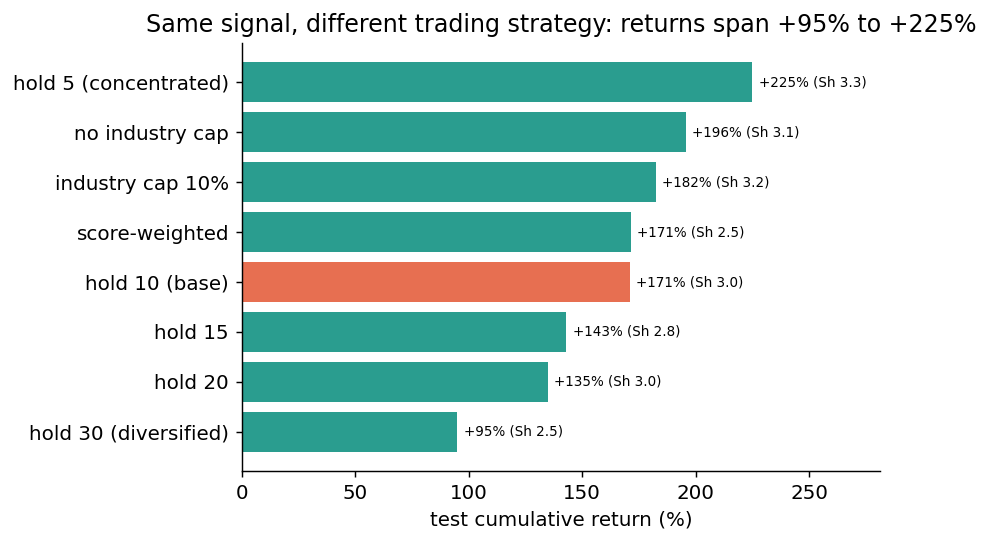
\includegraphics[width=0.82\linewidth]{figures/fig_strategy.png}
\caption{交易策略对收益的影响（固定同一组 base 预测）。同一信号在不同组合构建下收益从 $+95\%$ 到 $+225\%$；
持仓越集中收益越高（也越依赖个股），base（橙色）取持仓 $10$ 只的折中。括号内为 Sharpe。}
\label{fig:strategy}
\end{figure}

\begin{table}[H]
\centering
\caption{交易策略对收益的影响（固定 base 最优-ckpt 预测，test 期）。}
\label{tab:strategy}
\begin{tabular}{lcccc}
\toprule
策略 & 累计收益 & Sharpe & 最大回撤 & 换手率 \\
\midrule
持仓 5 只（集中）    & $+225.0\%$ & $3.34$ & $-16.0\%$ & $0.29$ \\
持仓 10 只（base）   & $+170.9\%$ & $2.99$ & $-14.7\%$ & $0.30$ \\
持仓 15 只           & $+143.0\%$ & $2.78$ & $-12.7\%$ & $0.31$ \\
持仓 20 只           & $+134.7\%$ & $2.96$ & $-11.3\%$ & $0.31$ \\
持仓 30 只（分散）   & $+94.9\%$  & $2.53$ & $-12.4\%$ & $0.32$ \\
分数加权（持仓 10）  & $+171.3\%$ & $2.53$ & $-17.2\%$ & $0.60$ \\
无行业上限           & $+195.5\%$ & $3.10$ & $-14.7\%$ & $0.31$ \\
行业上限 $10\%$      & $+182.3\%$ & $3.19$ & $-13.0\%$ & $0.31$ \\
\bottomrule
\end{tabular}
\end{table}

为考察深度版本在更集中口径下的表现，我们将报告支撑的深度版本置于
$n=5$、行业上限 $20\%$、掉出 Top-200 才换仓的口径下复测，
使用研究用 top1000 池、开盘成交与费用口径。结果见表~\ref{tab:release-strategy-sweep}：
M2.2/L5 在高集中策略下达到 $+354.59\%$。
配套的 benchmark runner（\path{scripts/benchmark_research.py}）在兼容的
top1000 研究面板上复现该口径，得到 $+354.34\%$、Sharpe $3.99$、最大回撤 $-17.68\%$。

\begin{table}[H]
\centering
\caption{公开模型的策略 sweep 补充结果（top1000 / 开盘成交 / 含费，固定预测只改组合规则）。}
\label{tab:release-strategy-sweep}
\begin{tabular}{lccccc}
\toprule
模型 & $n=5$, cap20 & $n=10$ base & $n=30$, cap20 & $n=10$, no cap & $n=10$, cap10 \\
\midrule
M2.1 / L4 seed42 ep17   & $+147.21\%$ & $+224.12\%$ & $+107.46\%$ & $+215.79\%$ & $+172.03\%$ \\
M2.2 / L5 seed2024 ep20 & $\mathbf{+354.59\%}$ & $+235.33\%$ & $+113.26\%$ & $+253.00\%$ & $+196.96\%$ \\
\bottomrule
\end{tabular}
\end{table}


\section{代码与复现说明}\label{sec:repro}
本文训练 / 推理 / benchmark 的公开入口如下。历史完整实验需要外部数据面板；仓库中的静态页面、checkpoint inference 和 baseline smoke path 可直接复现。
\begin{itemize}
  \item \textbf{\heiti 页面数据重建.} 兼容入口为 \path{build/update_daily.py}，实际调用 \path{build/update_research_live.py}，在兼容研究面板上重建 \path{docs/data/data.json} 中的 M-1-M/M-2-M 历史曲线。
  \item \textbf{\heiti Checkpoint 推理.} 入口为 \path{build/inference.py}，可对 M-1-M 与 M-2-M 两条公开研究曲线的 checkpoint 重新生成预测；单模型测试应写入临时路径，避免覆盖已提交缓存。
  \item \textbf{\heiti Research benchmark.} 入口为 \path{scripts/benchmark_research.py}，在兼容历史 top1000 面板与行业文件上复现研究回测口径；该路径是公开 benchmark 主口径。
  \item \textbf{\heiti Baseline 训练.} 公开训练入口是 \path{scripts/train_baseline.py} 与 \path{configs/baseline.json}。仓库提供 committed cache 上的 smoke test；完整 baseline 训练需要传入兼容 \path{docs/DATA_SCHEMA.md} 的历史面板。
  \item \textbf{\heiti 数据协议.} 完整研究数据不随仓库发布；公开仓库提供 BaoStock + AKShare + efinance 驱动的公开数据适配层、字段 schema 与 baseline 代码路径。若要复现实验表格，需要自行准备 2017--2026 区间、字段一致的 A 股日频面板。
  \item \textbf{\heiti 研究表格边界.} 本报告中的多种子、消融、可解释性与策略 sweep 表格是冻结研究记录。公开仓库保证方法、模型结构、benchmark runner 与 baseline reproduction path 可审计；完整历史研究表格的重跑依赖外部数据与算力。
  \item \textbf{\heiti 环境与随机性.} 推荐 Python~3.9+ 与 PyTorch。随机性由种子控制（\texttt{torch.manual\_seed} / \texttt{cuda.manual\_seed\_all}），但未承诺逐位确定性；因此研究结果应按多种子统计口径理解，而不是依赖单次运行。
\end{itemize}



% ================================================================ 参考文献
\begin{thebibliography}{99}
\small
\bibitem{lstm} S.~Hochreiter and J.~Schmidhuber. Long Short-Term Memory. \emph{Neural Computation}, 9(8):1735--1780, 1997.
\bibitem{alstm} Y.~Qin, D.~Song, H.~Cheng, W.~Cheng, G.~Jiang, and G.~W.~Cottrell. A Dual-Stage Attention-Based Recurrent Neural Network for Time Series Prediction. \emph{IJCAI}, 2017.
\bibitem{sfm} L.~Zhang, C.~Aggarwal, and G.-J.~Qi. Stock Price Prediction via Discovering Multi-Frequency Trading Patterns. \emph{KDD}, 2017.
\bibitem{transformer} A.~Vaswani et al. Attention Is All You Need. \emph{NeurIPS}, 2017.
\bibitem{rsr} F.~Feng, X.~He, X.~Wang, C.~Luo, Y.~Liu, and T.-S.~Chua. Temporal Relational Ranking for Stock Prediction. \emph{ACM Transactions on Information Systems (TOIS)}, 37(2):1--30, 2019.
\bibitem{advalstm} F.~Feng, H.~Chen, X.~He, J.~Ding, M.~Sun, and T.-S.~Chua. Enhancing Stock Movement Prediction with Adversarial Training. \emph{IJCAI}, 2019.
\bibitem{dtml} J.~Yoo, Y.~Soun, Y.-c.~Park, and U.~Kang. Accurate Multivariate Stock Movement Prediction via Data-Axis Transformer with Multi-Level Contexts. \emph{KDD}, 2021.
\bibitem{tra} H.~Lin, D.~Zhou, W.~Liu, and J.~Bian. Learning Multiple Stock Trading Patterns with Temporal Routing Adaptor and Optimal Transport. \emph{KDD}, 2021.
\bibitem{hist} W.~Xu, W.~Liu, L.~Wang, Y.~Xia, J.~Bian, J.~Yin, and T.-Y.~Liu. HIST: A Graph-based Framework for Stock Trend Forecasting via Mining Concept-Oriented Shared Information. \emph{arXiv:2110.13716}, 2021.
\bibitem{crossformer} Y.~Zhang and J.~Yan. Crossformer: Transformer Utilizing Cross-Dimension Dependency for Multivariate Time Series Forecasting. \emph{ICLR}, 2023.
\bibitem{stockmixer} J.~Fan and Y.~Shen. StockMixer: A Simple yet Strong MLP-based Architecture for Stock Price Forecasting. \emph{AAAI}, 2024.
\bibitem{master} T.~Li, Z.~Liu, Y.~Shen, X.~Wang, H.~Chen, and S.~Xiong. MASTER: Market-Guided Stock Transformer for Stock Price Forecasting. \emph{AAAI}, 2024.
\bibitem{gausstransformer} Q.~Ding, S.~Wu, H.~Sun, J.~Guo, and J.~Guo. Hierarchical Multi-Scale Gaussian Transformer for Stock Movement Prediction. \emph{IJCAI}, 2020.
\bibitem{survey} L.~Cao, et al. From Deep Learning to LLMs: A Survey of AI in Quantitative Investment. \emph{arXiv:2503.21422}, 2025.
\bibitem{qlib} X.~Yang, W.~Liu, D.~Zhou, J.~Bian, and T.-Y.~Liu. Qlib: An AI-oriented Quantitative Investment Platform. \emph{arXiv:2009.11189}, 2020.（Alpha158 因子库来源，\texttt{microsoft/qlib}）
\end{thebibliography}

\end{document}
